% Presets
\setbeamertemplate{itemize/enumerate body begin}{\footnotesize}
\setbeamertemplate{itemize/enumerate subbody begin}{\footnotesize}




%%%%%%%%%%%%%%%%%%%%%%%%%%%%%%%%%%%%%%%%%%%%%%%%%%%%%%%%%%%%%%%%%%%%%%%%%%%%%%%%%%%%%%%%%%%%%%%%%%%%%%%%%%%%%%%%%%%%%%%%%%%%
% Title page
%%%%%%%%%%%%%%%%%%%%%%%%%%%%%%%%%%%%%%%%%%%%%%%%%%%%%%%%%%%%%%%%%%%%%%%%%%%%%%%%%%%%%%%%%%%%%%%%%%%%%%%%%%%%%%%%%%%%%%%%%%%%


% Create background image
{\setbeamertemplate{sidebar right}{\llap{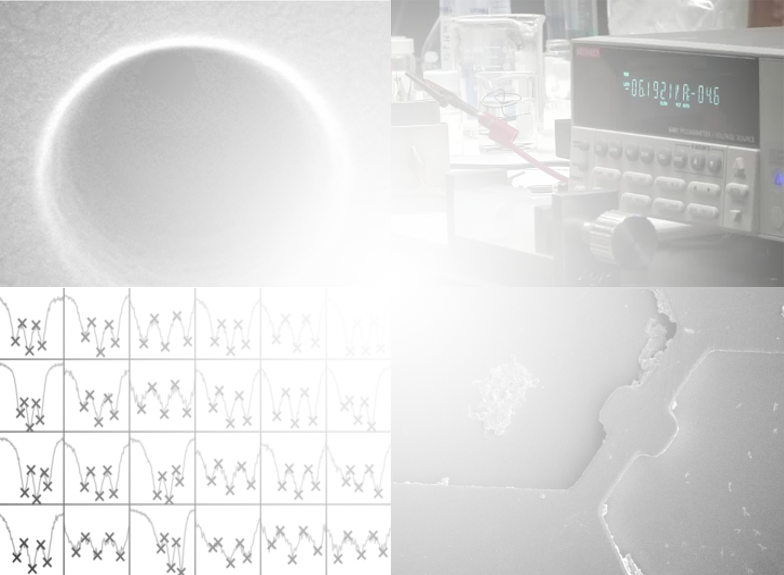
\includegraphics[width=\paperwidth,height=\paperheight]{title_image.png}}}
\begin{frame}[c]
 \begin{center}
  

  
  % Title
  \Huge{
	\textcolor{gray0}{Resistive-pulse sensing at the micro- and nanoscale}
  }
  
  
  % Name --- Institution
  \vspace{.25in}
  {\Large 
	\textcolor{gray1}{Preston Hinkle} \hspace{.5in} 
\includegraphics[height=1em]{uci_wordmark.png}
  }
  
  
  % Talk location
  \vspace{.5in}
  {\small
	\textit{\today}
  }
  
  
  
 \end{center}

\end{frame}
}



%%%%%%%%%%%%%%%%%%%%%%%%%%%%%%%%%%%%%%%%%%%%%%%%%%%%%%%%%%%%%%%%%%%%%%%%%%%%%%%%%%%%%%%%%%%%%%%%%%%%%%%%%%%%%%%%%%%%%%%%%%%%
% Outline
%%%%%%%%%%%%%%%%%%%%%%%%%%%%%%%%%%%%%%%%%%%%%%%%%%%%%%%%%%%%%%%%%%%%%%%%%%%%%%%%%%%%%%%%%%%%%%%%%%%%%%%%%%%%%%%%%%%%%%%%%%%%


\begin{frame}[c]{Outline}
 
	\begin{columns}[t]
		\begin{column}[T]{2.25in}
		
			\setbeamercovered{transparent}
			\begin{itemize}
				\item\only<1>{\textcolor{porestatsblack}{Resistive pulse sensing background}}\only<2,3,4>{\textcolor{ucigray0}{Resistive pulse sensing background}}
				\item\only<2>{\textcolor{porestatsblack}{Resistive pulse sensing of high-aspect ratio particles}}\only<1,3,4>{\textcolor{ucigray0}{Resistive pulse sensing of high-aspect ratio particles}}	
				\item\only<3,4>{\textcolor{porestatsblack}{Microscale resistive pulse sensing}}\only<1,2>{\textcolor{ucigray0}{Microscale resistive pulse sensing}}
				
					\begin{itemize}
						\item\only<3>{\textcolor{porestatsblack}{Simultaneous imaging and resistive pulse studies}}\only<1,2,4>{\textcolor{ucigray0}{Simultaneous imaging and resistive pulse studies}}
						\item\only<4>{\textcolor{porestatsblack}{Cancer cell deformability cytometry}}\only<1,2,3>{\textcolor{ucigray0}{Cancer cell deformability cytometry}}
					\end{itemize}
					
					
				
			\end{itemize}
			\setbeamercovered{invisible}
			
		\end{column}
		
		
		\begin{column}[T]{2.25in}
	
		
			% RP Background 1
			\onslide<1>{
				\begin{picture}(0,0)(0,0)
					\put(0,-180)
					{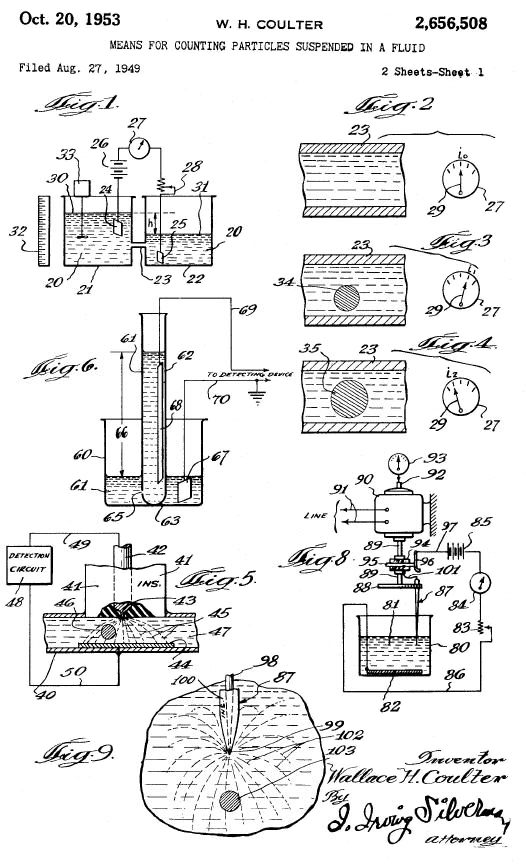
\includegraphics[width=2in]{coulter_patent_drawing}}
				\end{picture}
			}

		
			% Rods 1
			\onslide<2>{
				\begin{picture}(0,0)(0,0)
					\put(10,-30)
					{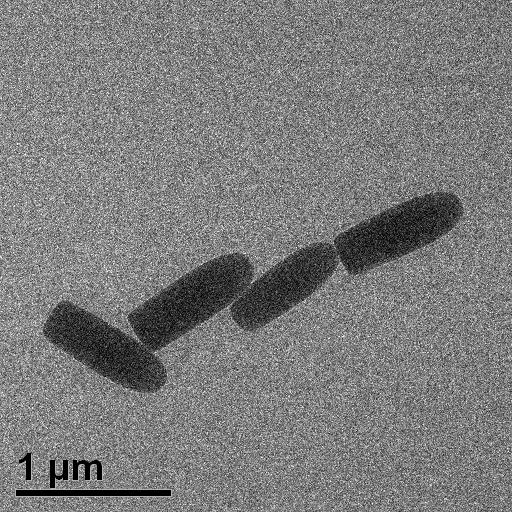
\includegraphics[width=1.25in]{shortrods}}
				\end{picture}
			}
			
			% Rods 2
			\onslide<2>{
				\begin{picture}(0,0)(0,0)
					\put(50,-125)
					{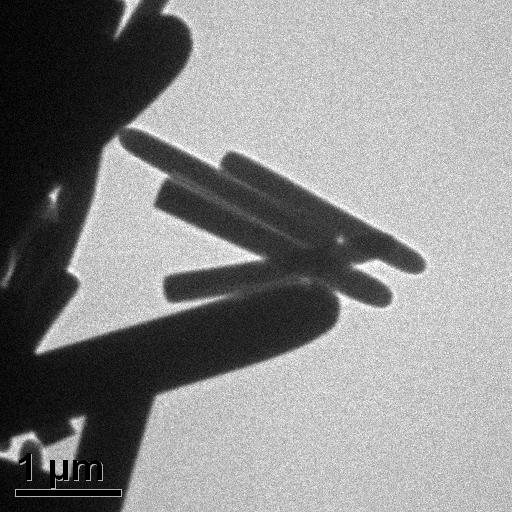
\includegraphics[width=1.25in]{longrods}}
				\end{picture}
			}
			
			
			% RPIM 1
			\onslide<3>{
				\begin{picture}(0,0)(0,0)
					\put(0, -65)
					{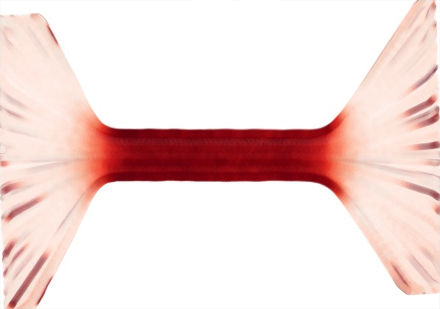
\includegraphics[width=2.25in]{resistancemap}}
				\end{picture}
			}
			
			% Cells
			\onslide<4>{
				\begin{picture}(0,0)(0,0)
					\put(0, -75)
					{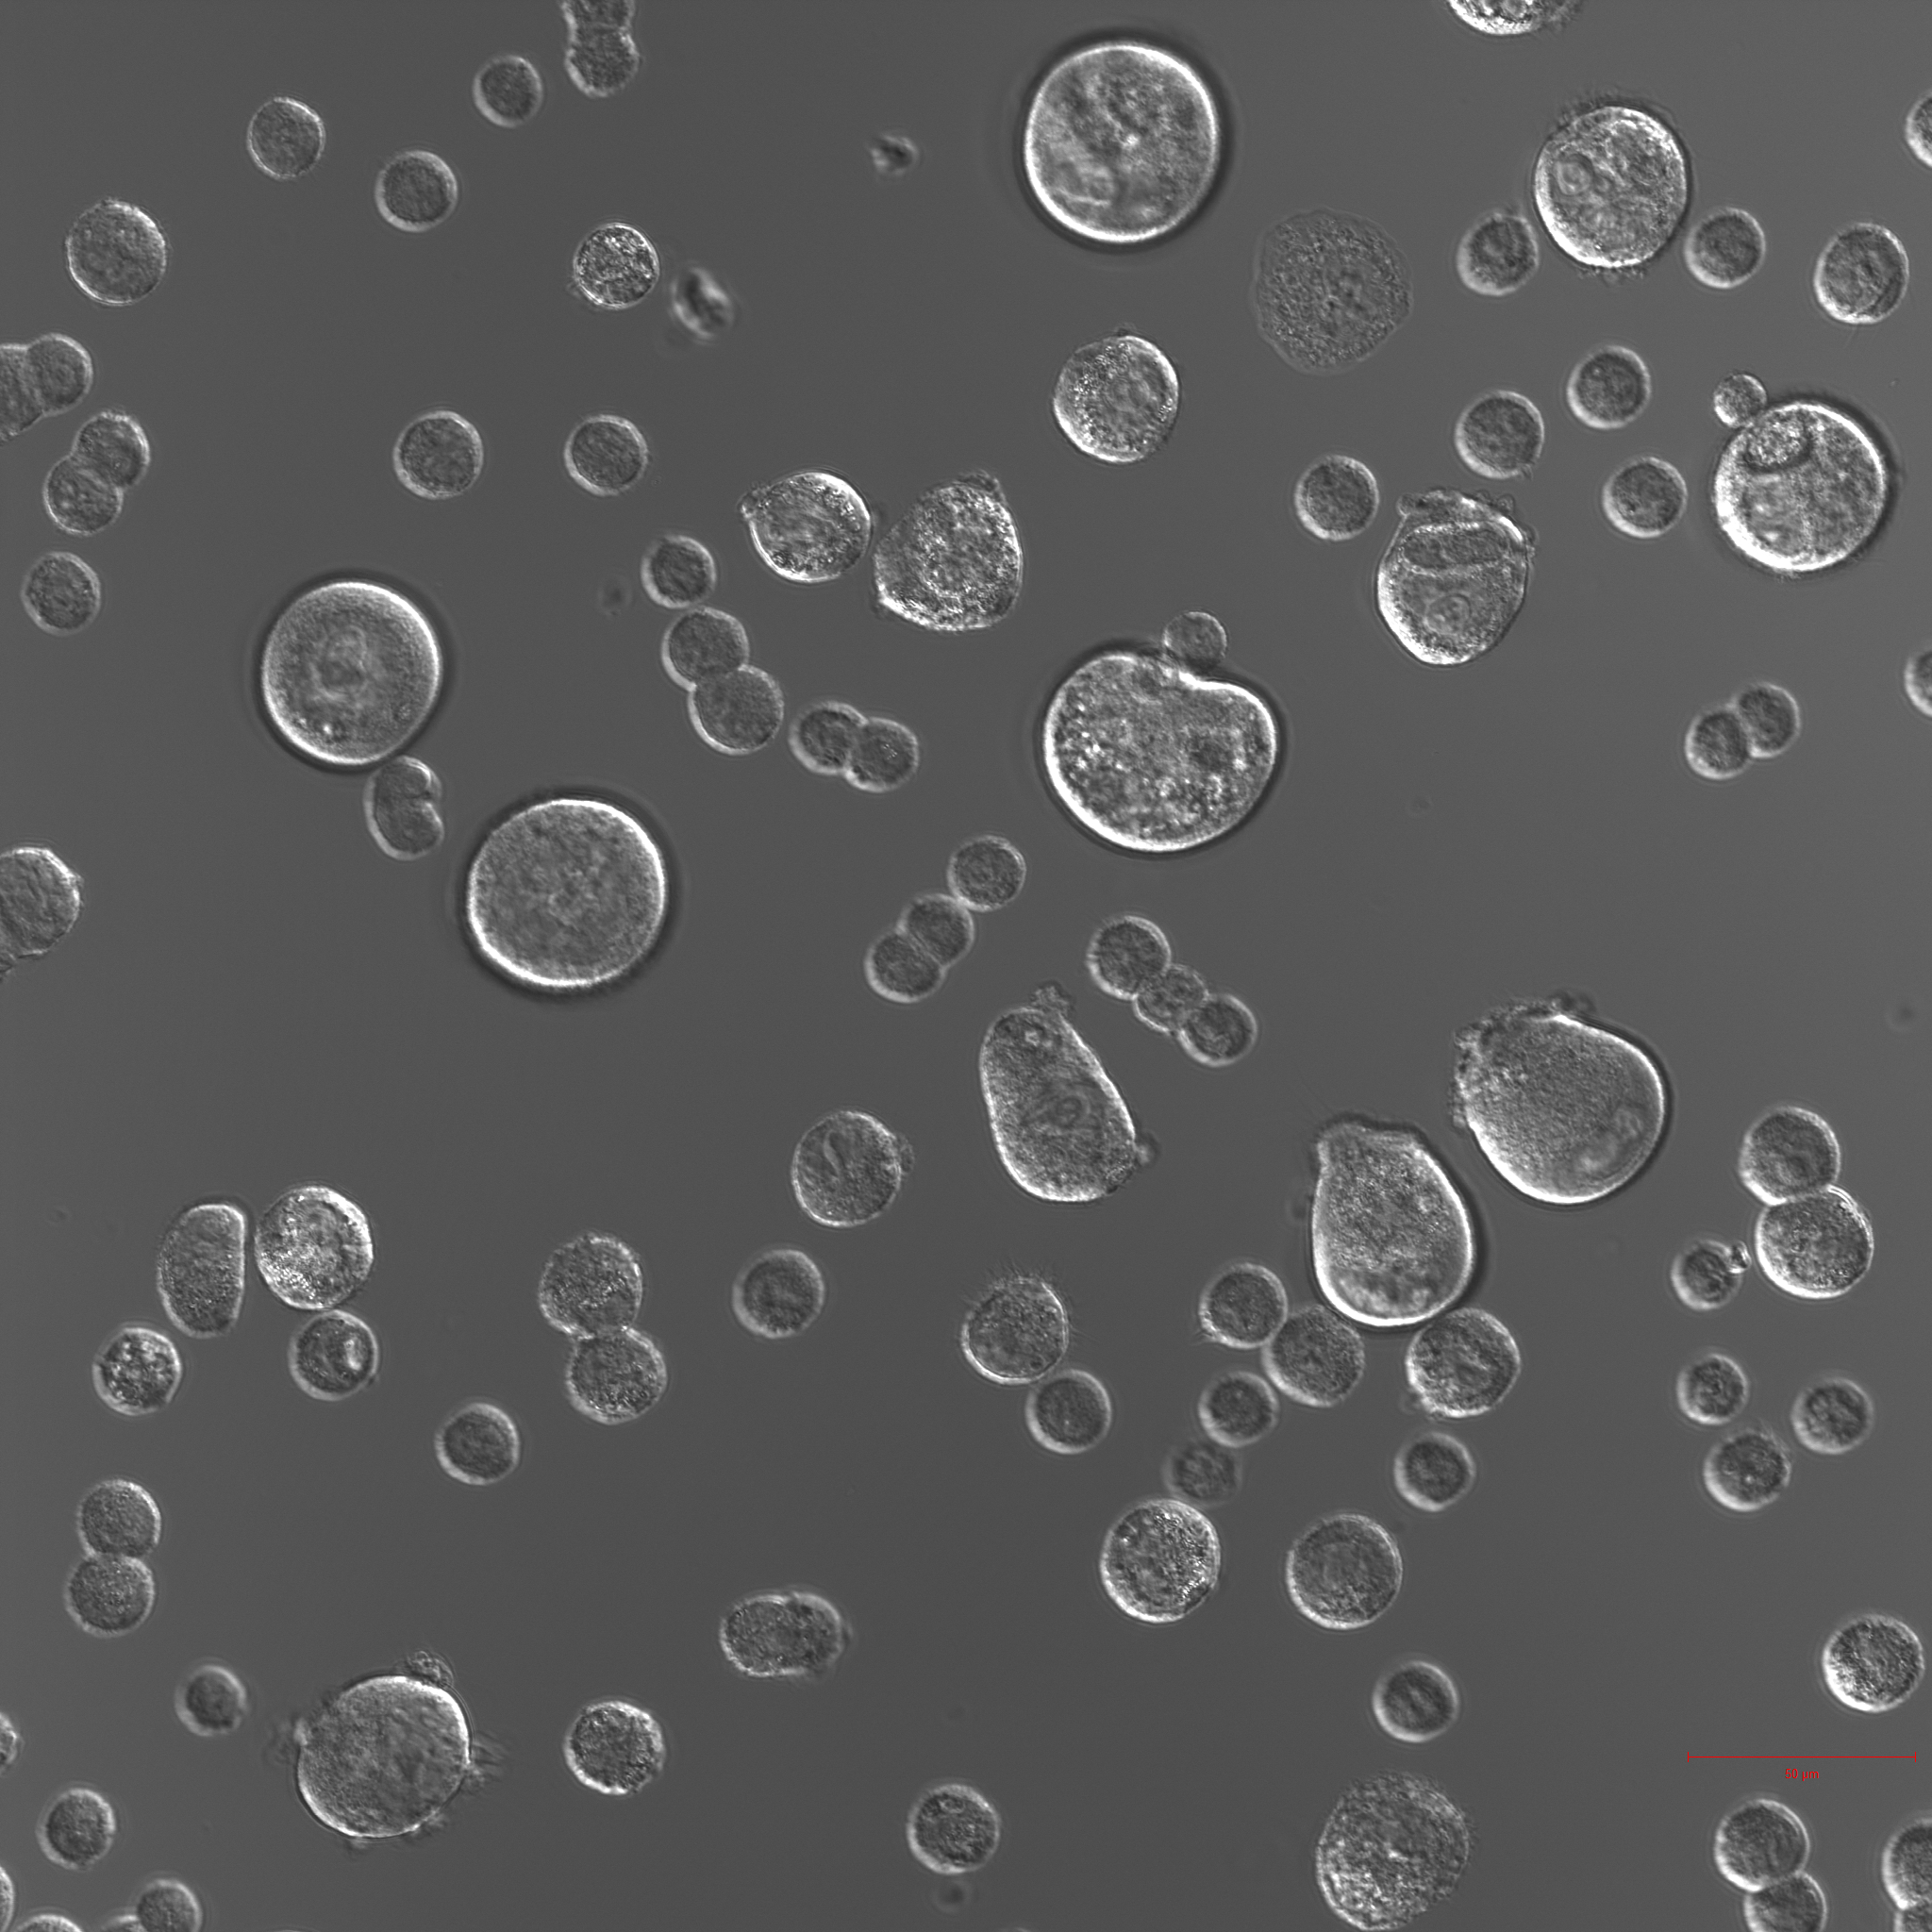
\includegraphics[width=2.25in]{cells}}
				\end{picture}
			}


			
			
		\end{column}
		
	\end{columns}

	
	
	
	
	
\end{frame}


%%%%%%%%%%%%%%%%%%%%%%%%%%%%%%%%%%%%%%%%%%%%%%%%%%%%%%%%%%%%%%%%%%%%%%%%%%%%%%%%%%%%%%%%%%%%%%%%%%%%%%%%%%%%%%%%%%%%%%%%%%%%
% Resistive pulse background title slide
%%%%%%%%%%%%%%%%%%%%%%%%%%%%%%%%%%%%%%%%%%%%%%%%%%%%%%%%%%%%%%%%%%%%%%%%%%%%%%%%%%%%%%%%%%%%%%%%%%%%%%%%%%%%%%%%%%%%%%%%%%%%


\begin{frame}[c]{}
	\begin{center}
		\textbf{Resistive pulse sensing background}
	\end{center}
\end{frame}



%%%%%%%%%%%%%%%%%%%%%%%%%%%%%%%%%%%%%%%%%%%%%%%%%%%%%%%%%%%%%%%%%%%%%%%%%%%%%%%%%%%%%%%%%%%%%%%%%%%%%%%%%%%%%%%%%%%%%%%%%%%%
% Resistive pulse background---description
%%%%%%%%%%%%%%%%%%%%%%%%%%%%%%%%%%%%%%%%%%%%%%%%%%%%%%%%%%%%%%%%%%%%%%%%%%%%%%%%%%%%%%%%%%%%%%%%%%%%%%%%%%%%%%%%%%%%%%%%%%%%


\begin{frame}[c]{Resistive pulse sensing---description}
	
	\begin{columns}[t]
		\begin{column}[T]{2.75in}
	
			\begin{itemize}
				\item Resistive pulse sensing (RP) is a method for single particle detection and characterization
				\item Works at any scale (nano, micro, milli, etc.)
				\item A diverse range of applications: red blood cell counting (several $\SI{}{\mu m}$, virus detection ($10-\SI{100}{\mu m}$, and DNA sequencing ($\sim\SI{1}{nm}$), among others
			\end{itemize}
	
		\end{column}
		
		\begin{column}[T]{1.75in}
			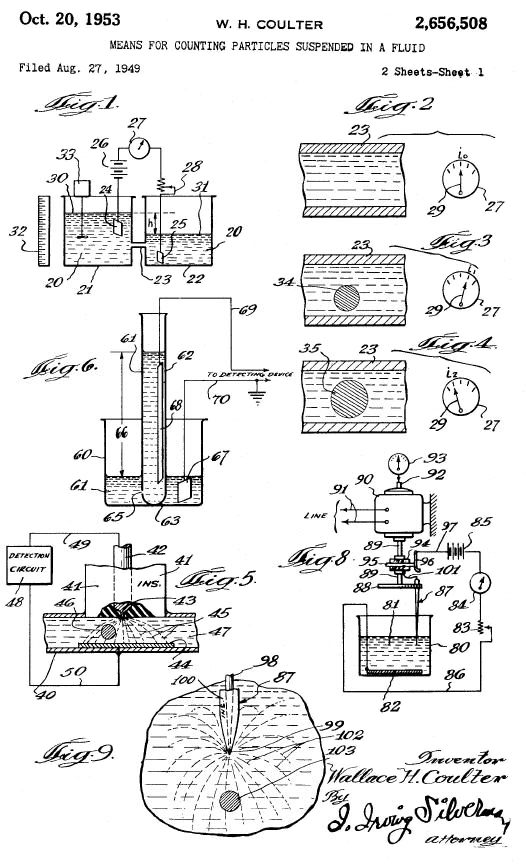
\includegraphics[width=1.75in]{coulter_patent_drawing.png}
		\end{column}
		
	\end{columns}

	
\end{frame}



%%%%%%%%%%%%%%%%%%%%%%%%%%%%%%%%%%%%%%%%%%%%%%%%%%%%%%%%%%%%%%%%%%%%%%%%%%%%%%%%%%%%%%%%%%%%%%%%%%%%%%%%%%%%%%%%%%%%%%%%%%%%
% Resistive pulse background---how does it work?
%%%%%%%%%%%%%%%%%%%%%%%%%%%%%%%%%%%%%%%%%%%%%%%%%%%%%%%%%%%%%%%%%%%%%%%%%%%%%%%%%%%%%%%%%%%%%%%%%%%%%%%%%%%%%%%%%%%%%%%%%%%%


\begin{frame}[c]{Resistive pulse sensing---how does it work?}

	\begin{columns}[t]
		\begin{column}[T]{2.75in}
	      
	

			\begin{tiny}
				\begin{itemize}
				
					\item A nanopore immersed in electrolyte solution acts as an ionic resistor
					\item Current-Voltage relationship follows Ohm's law $V=IR$
					\item When a particle enters the channel its resistance changes, yielding a pulse in the measured ionic current
					\item Pulse properties yield information on size, shape, charge, and concentration of particle
				\end{itemize}
				{\centering
					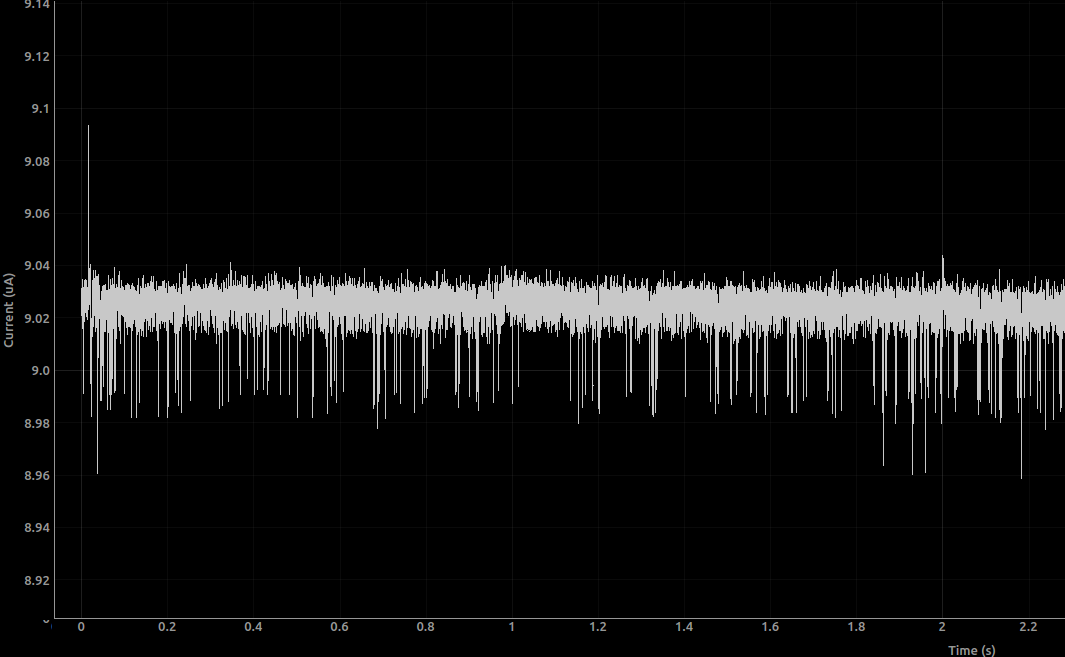
\includegraphics[height=1in,width=2.5in]{rp_timeseries.png} \\ \par
				}
			\end{tiny}
			
		\end{column}
		
		\begin{column}[T]{1.75in}
			{\centering
				\vspace{.5cm}
				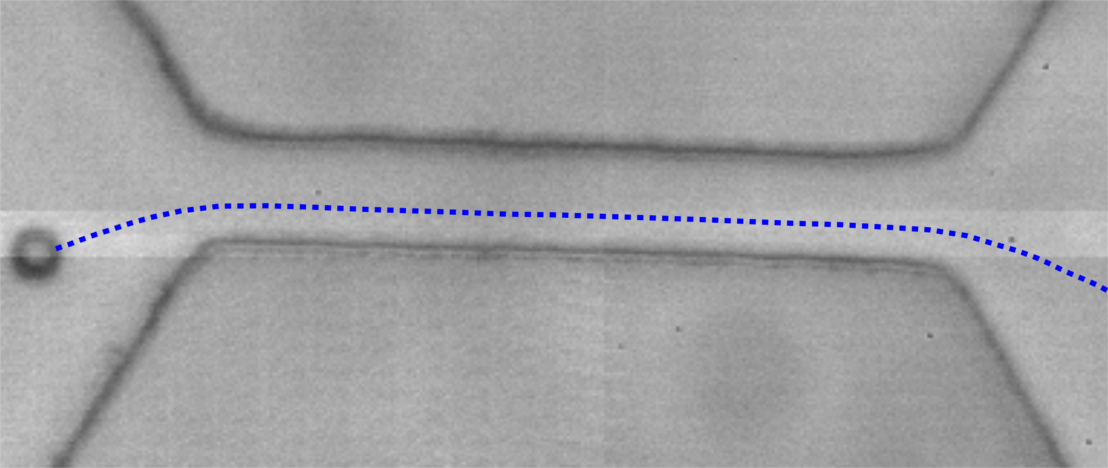
\includegraphics[width=1.5in]{singletrajectory} \\
				\vspace{.75cm}
				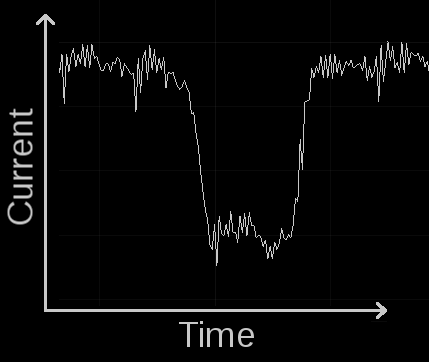
\includegraphics[width=1.5in]{singlerp} \\
				\par
			}
			
		\end{column}

	
	
	\end{columns}
	
\end{frame}




%%%%%%%%%%%%%%%%%%%%%%%%%%%%%%%%%%%%%%%%%%%%%%%%%%%%%%%%%%%%%%%%%%%%%%%%%%%%%%%%%%%%%%%%%%%%%%%%%%%%%%%%%%%%%%%%%%%%%%%%%%%%
% Resistive pulse background---system components
%%%%%%%%%%%%%%%%%%%%%%%%%%%%%%%%%%%%%%%%%%%%%%%%%%%%%%%%%%%%%%%%%%%%%%%%%%%%%%%%%%%%%%%%%%%%%%%%%%%%%%%%%%%%%%%%%%%%%%%%%%%%


\begin{frame}[c]{Resistive pulse sensing---system components}
	%\begin{picture}(0,0)(0,0)
		%\put(90,-125){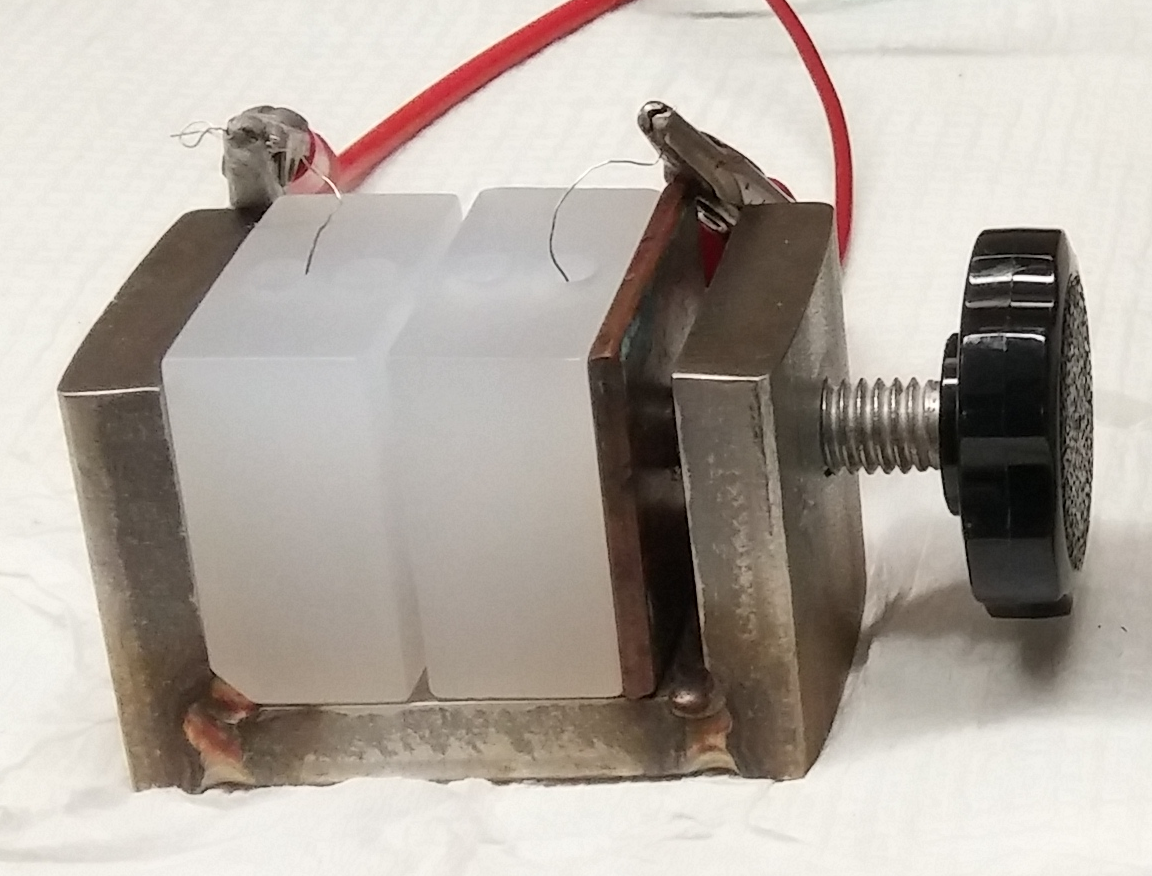
\includegraphics[width=7cm]{photo/conductivitycell.png}}
		%\put(100,0){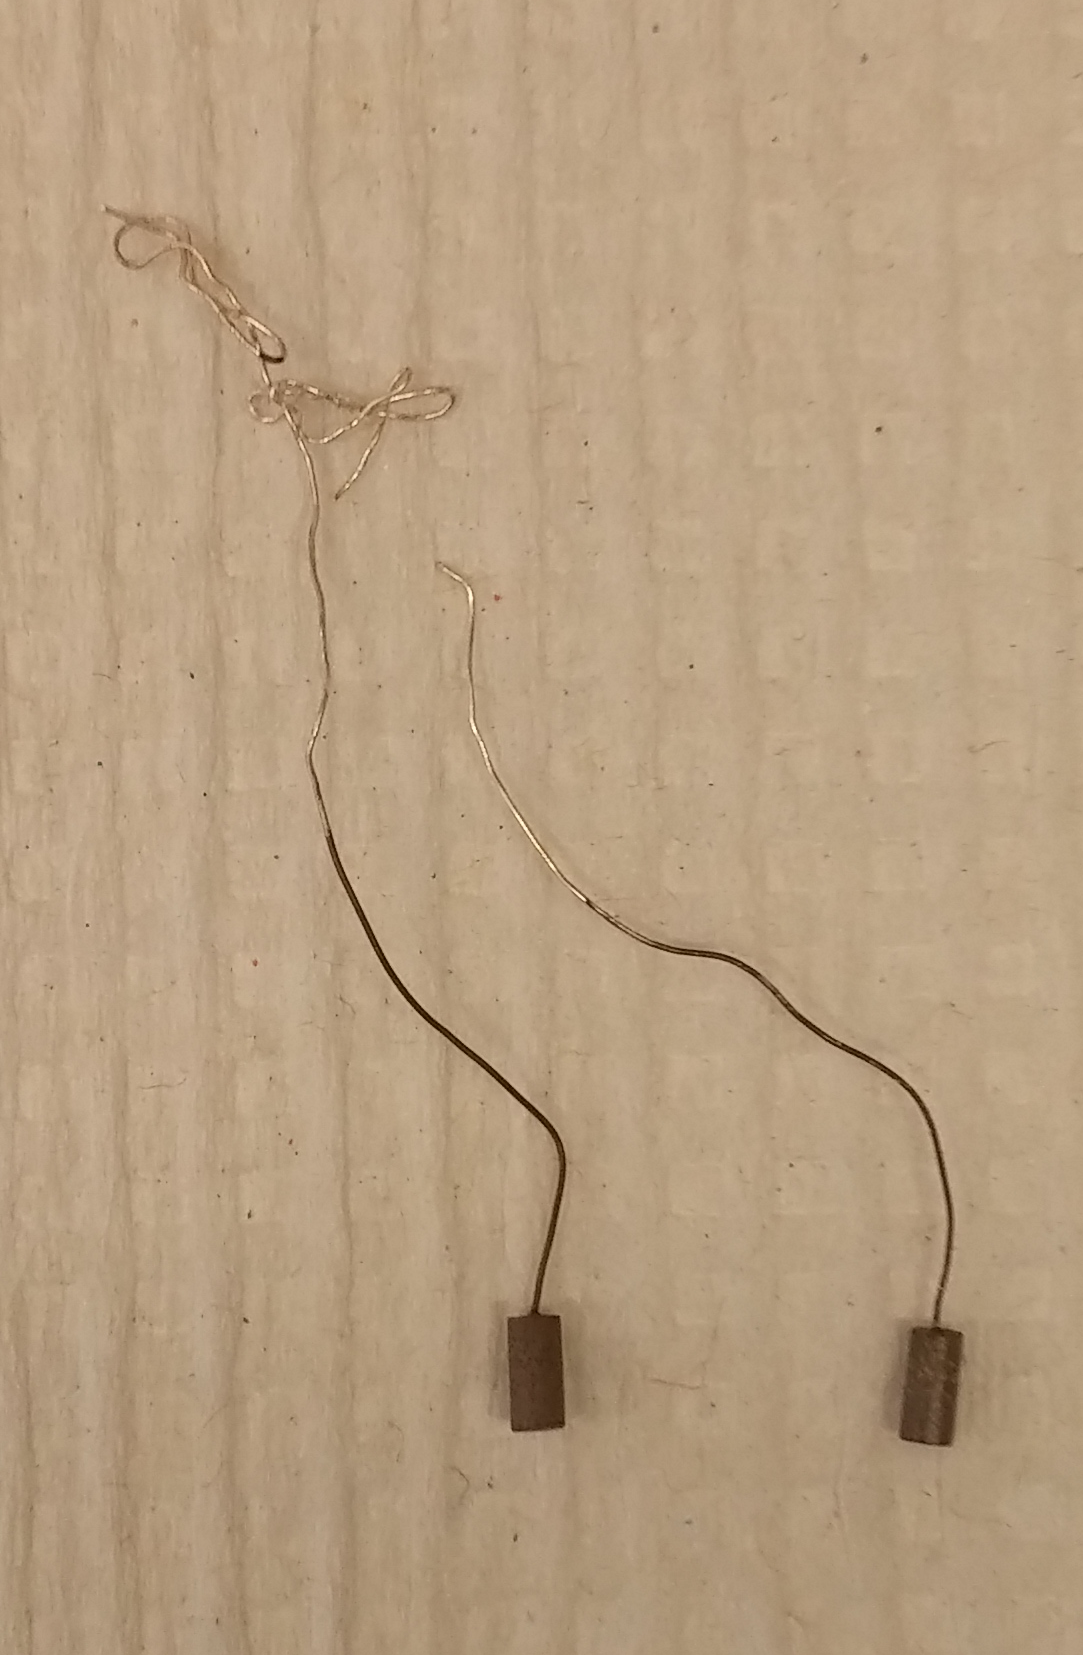
\includegraphics[width=2cm]{photo/electrodes.png}}
		%\put(10,-20){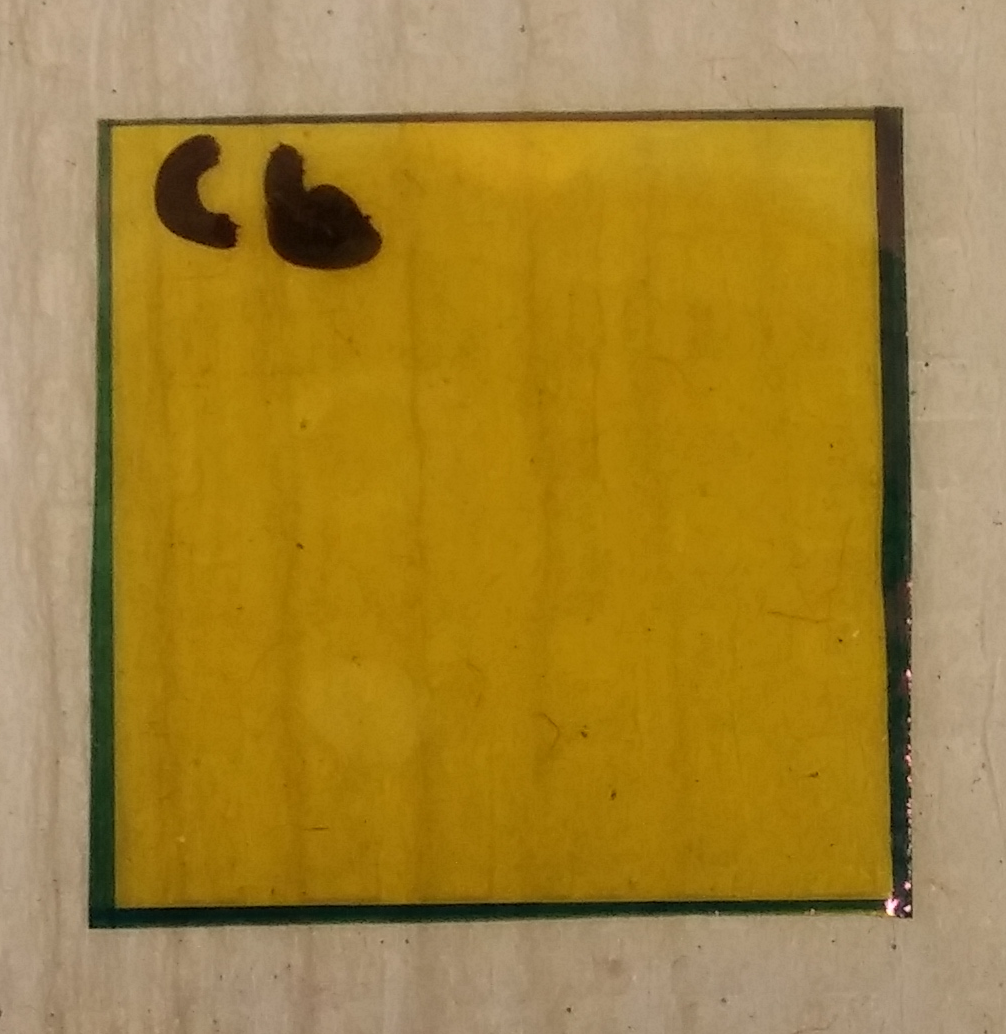
\includegraphics[width=2cm]{photo/membrane.png}}
		%\put(30,-80){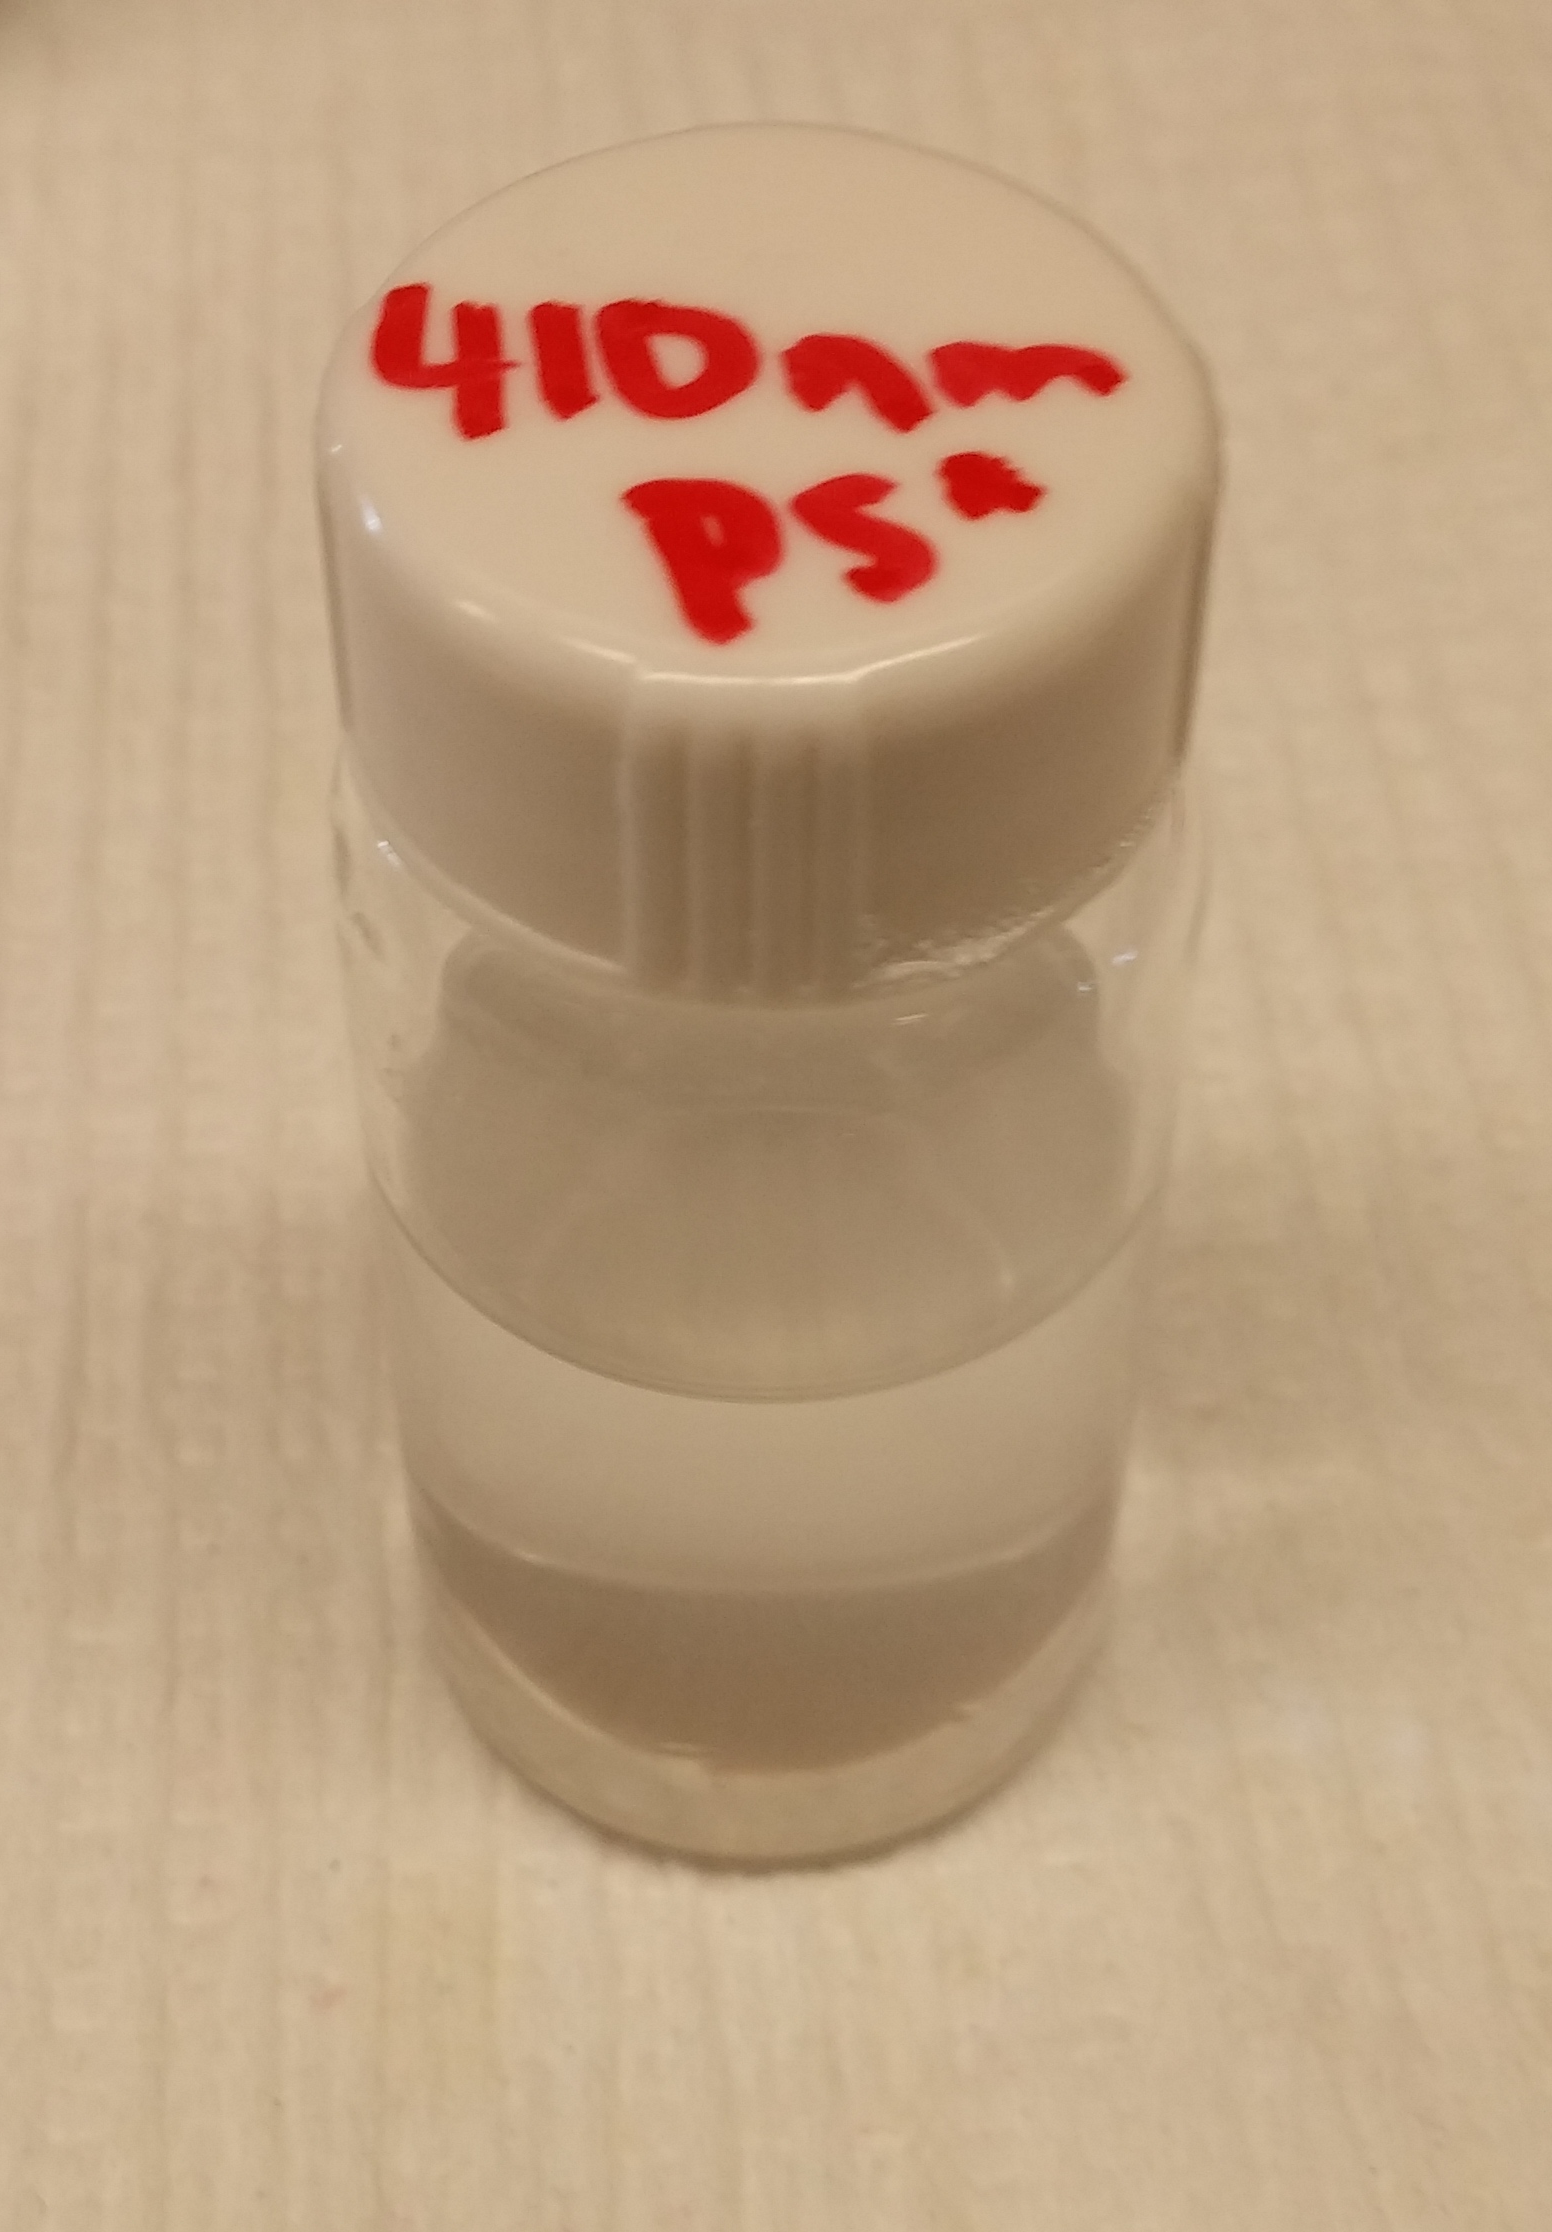
\includegraphics[width=2cm]{photo/solution.png}}
	%\end{picture}
% 	{\centering 
% 		\vspace{0.35cm}
% 		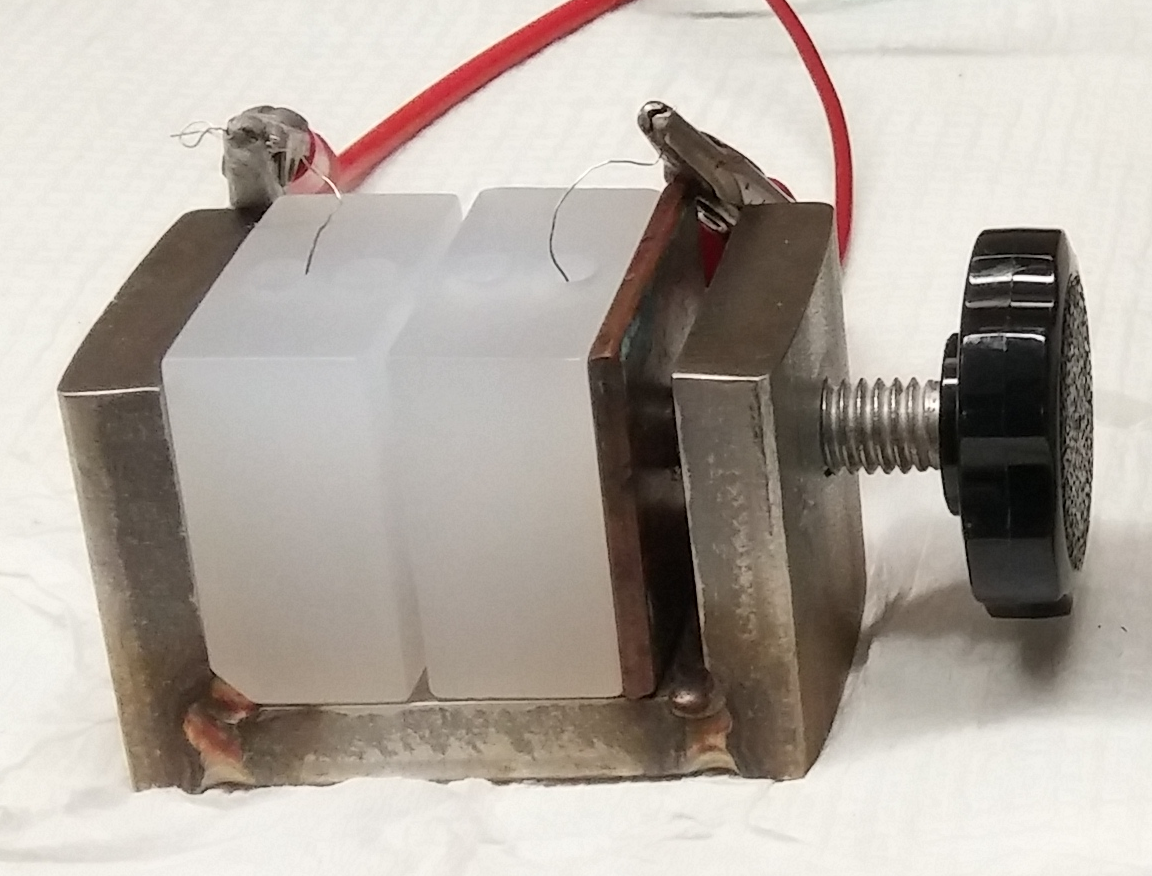
\includegraphics[width=9cm]{photo/conductivitycell.png}
% 		\newline
% 		\vspace{.35cm}
% 		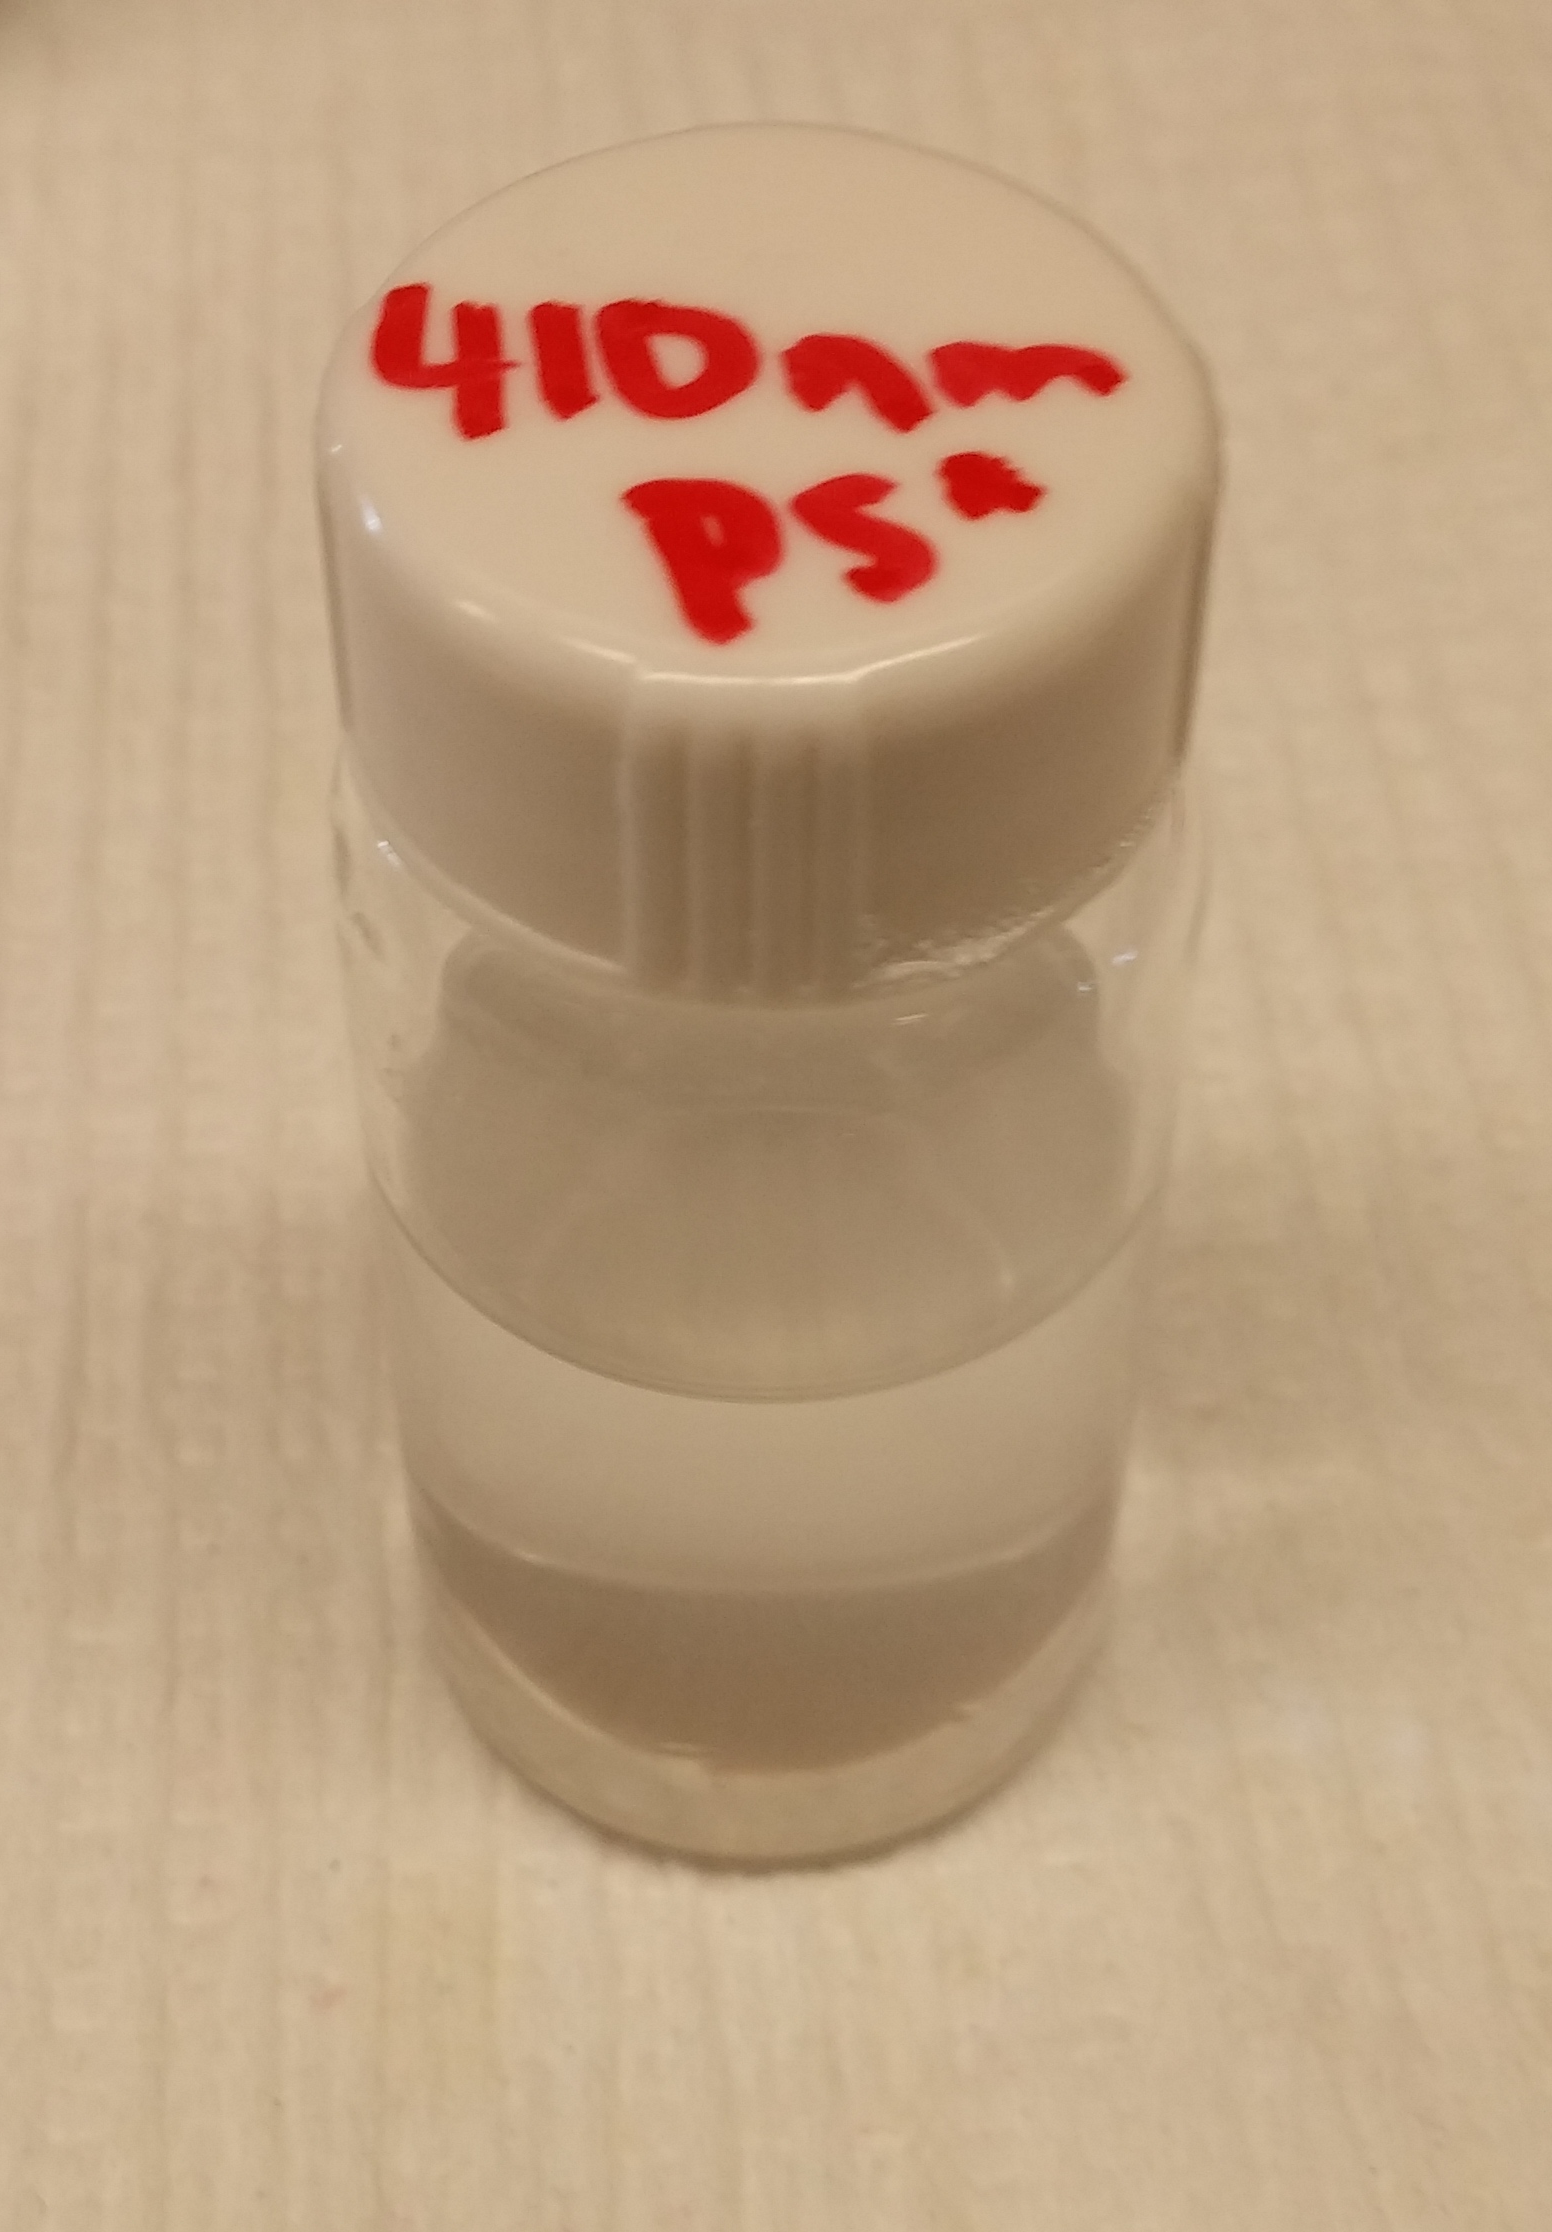
\includegraphics[width=1.5cm]{photo/solution.png}
% 		\hspace{1cm}
% 		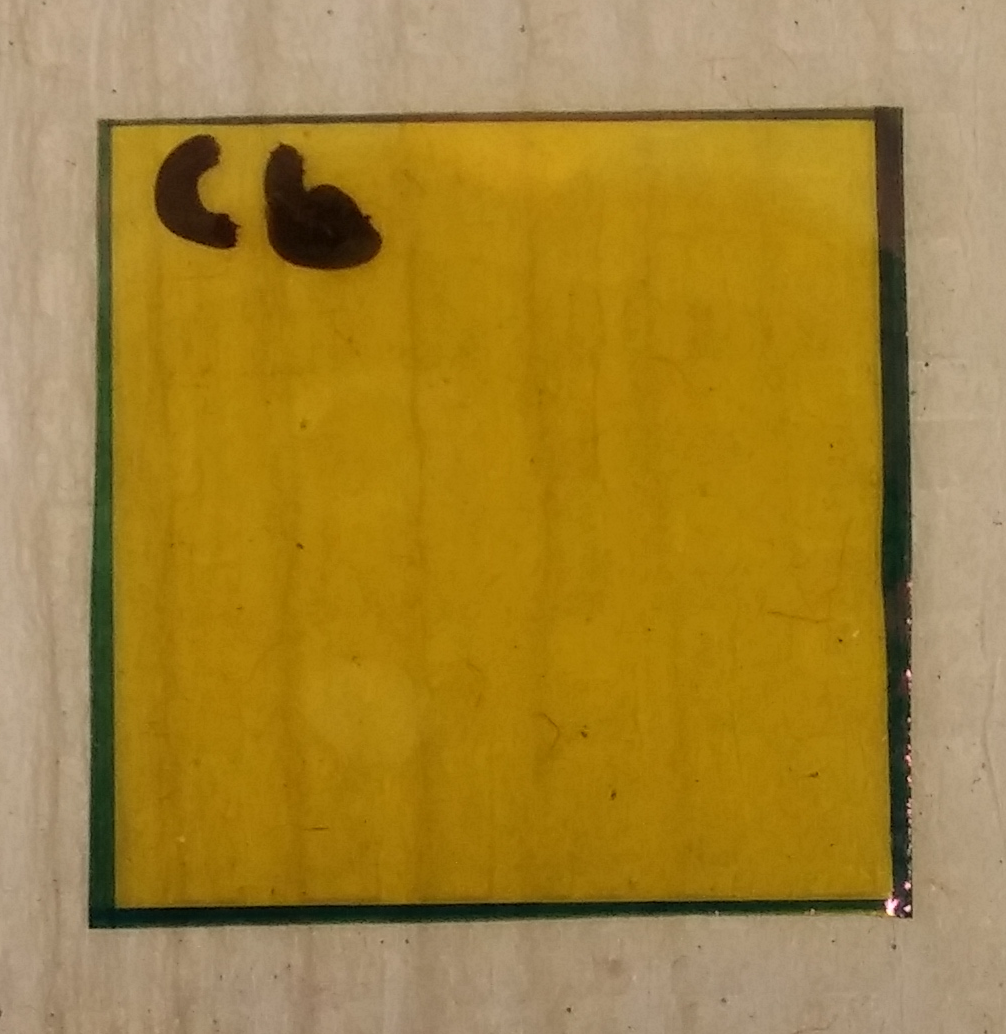
\includegraphics[width=2cm]{photo/membrane.png}
% 		\hspace{1cm}
% 		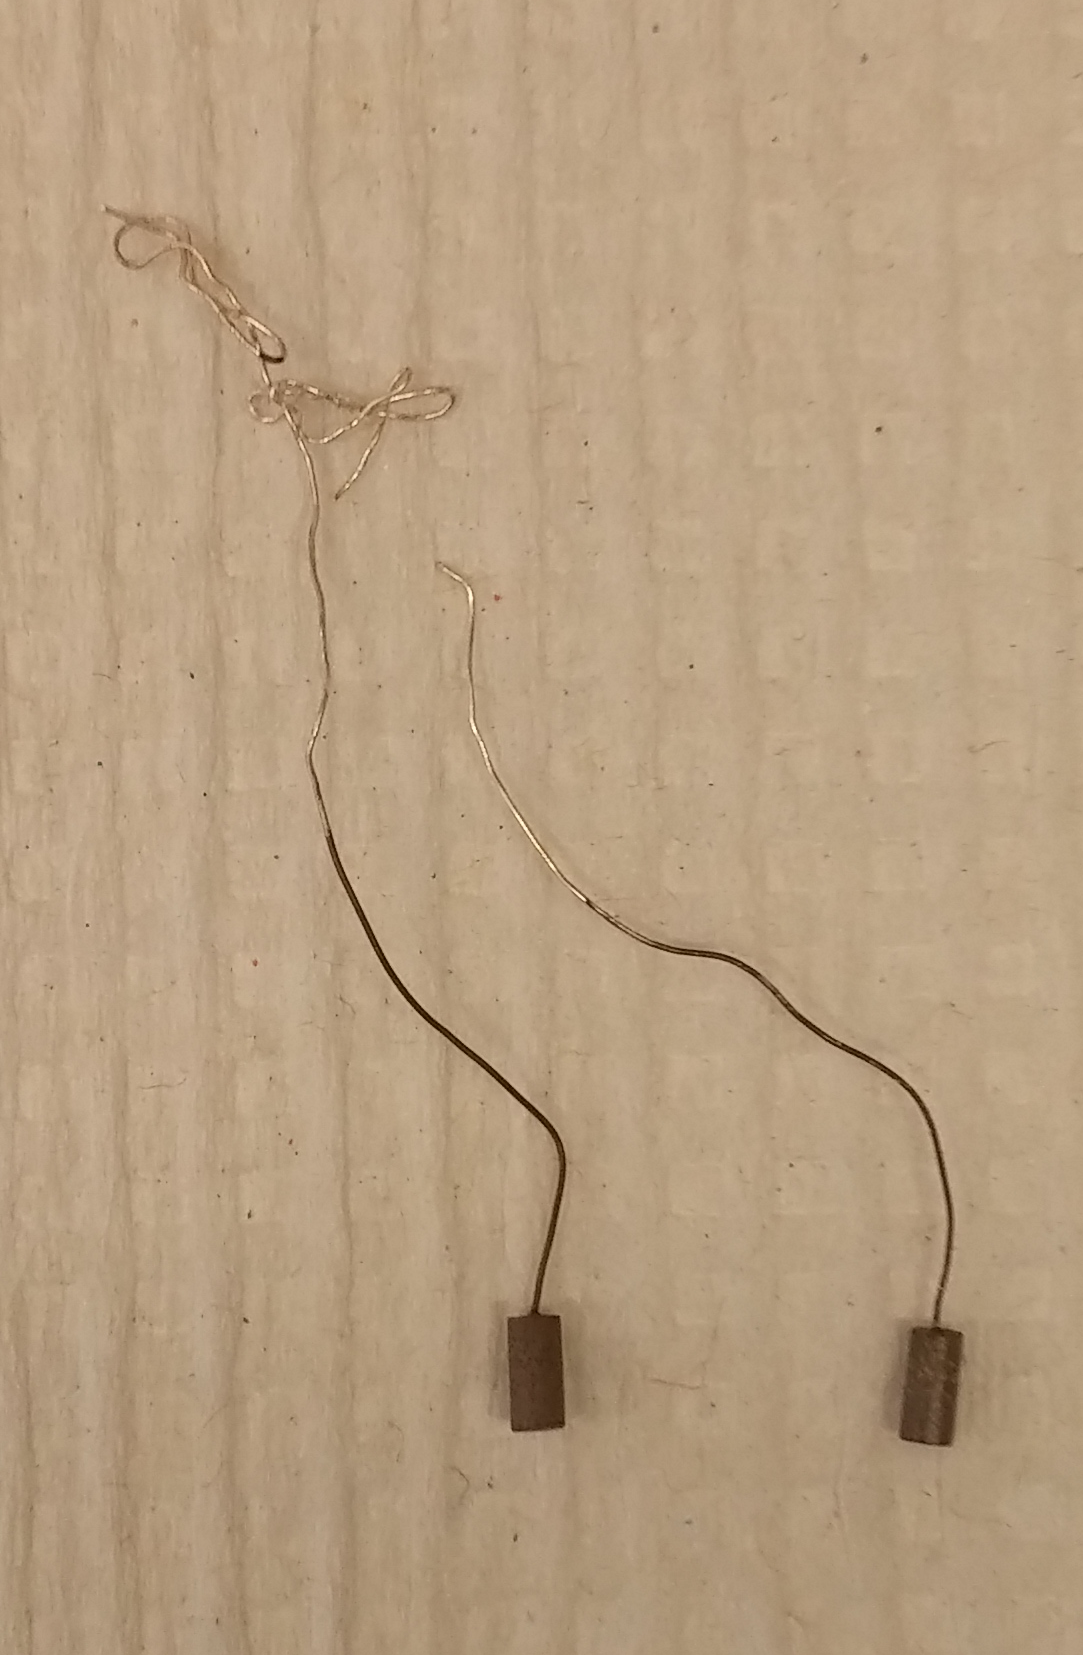
\includegraphics[width=1.5cm]{photo/electrodes.png}
% 		\hspace{1cm}
% 		\par
% 	}


	\begin{columns}[t]
		\begin{column}[T]{\paperwidth/5}
			{\centering
				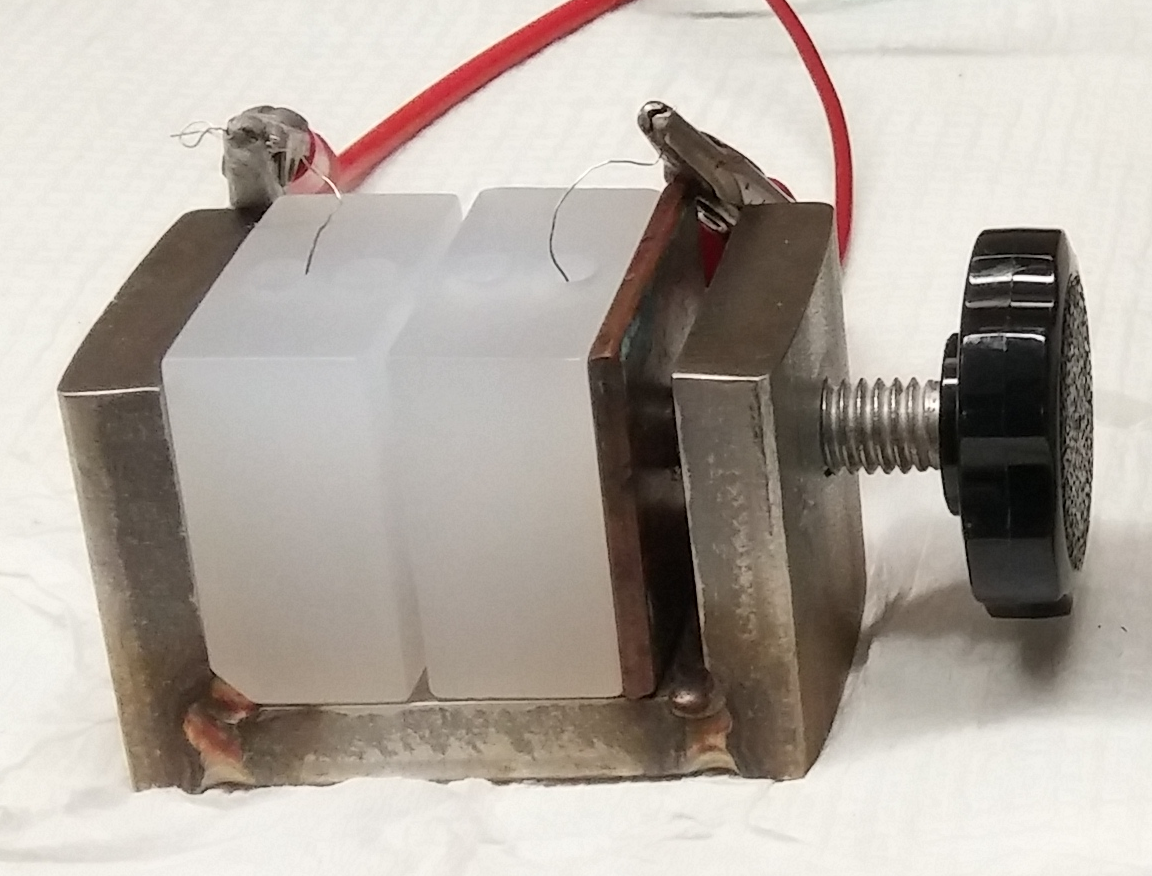
\includegraphics[height=2.25cm]{photo/conductivitycell.png} \\
				{\footnotesize Conductivity cell}
				\par
			}
		\end{column}
		
		
		\begin{column}[T]{\paperwidth/5}
			{\centering
				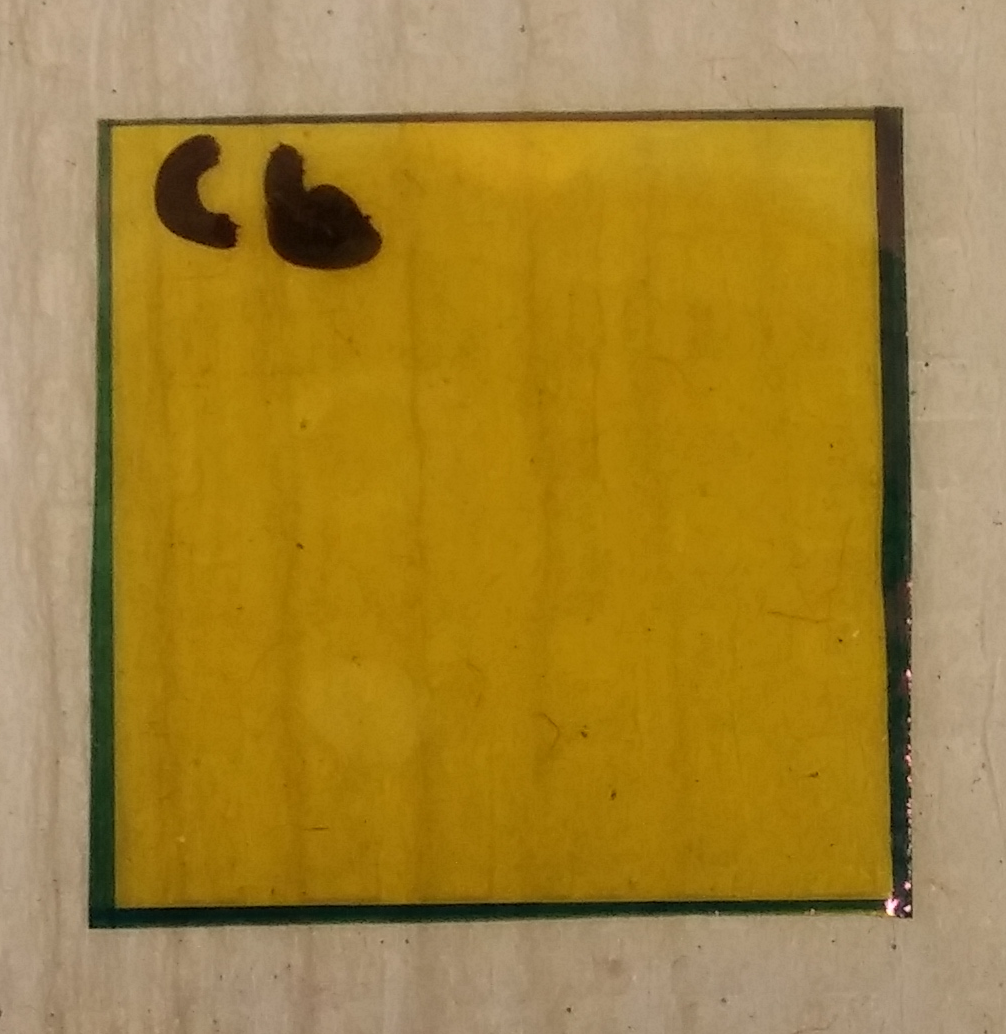
\includegraphics[height=2.25cm]{photo/membrane.png} \\
				{\footnotesize Pore membrane}
				\par
			}
		\end{column}
		
		
		
		\begin{column}[T]{\paperwidth/5}
			{\centering
				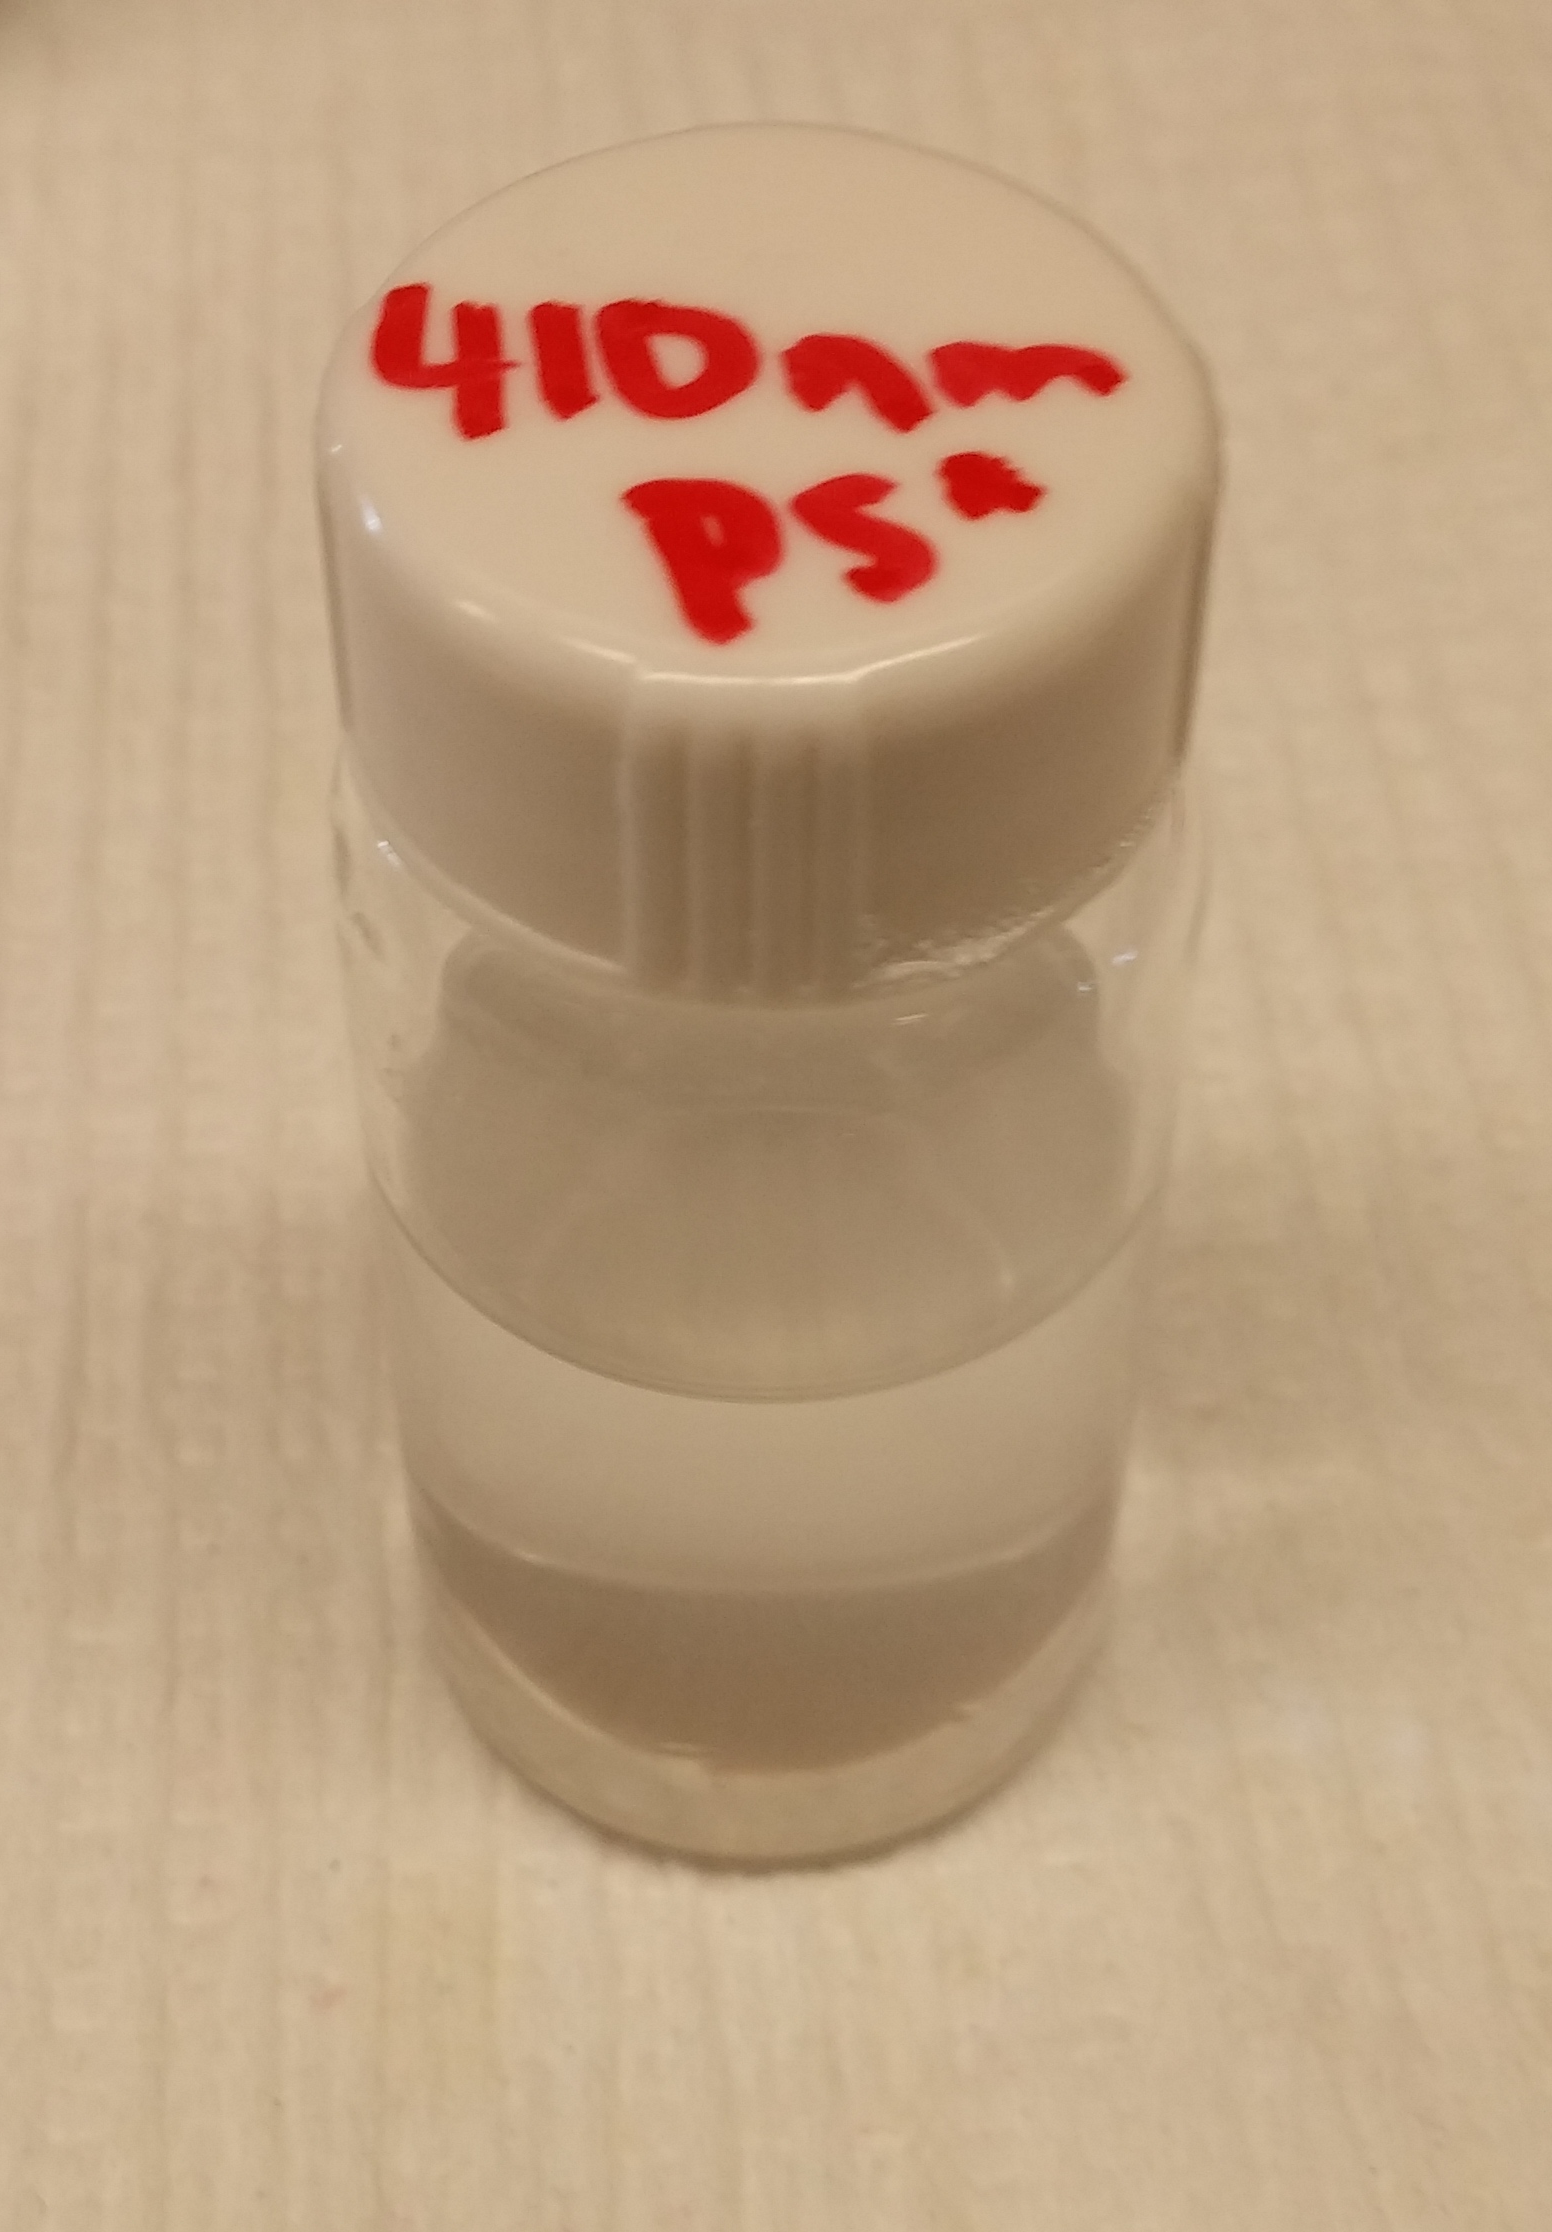
\includegraphics[height=2.25cm]{photo/solution.png} \\
				{\footnotesize Electrolyte}
				\par
			}
		\end{column}

		
		

		
		\begin{column}[T]{\paperwidth/5}
			{\centering
				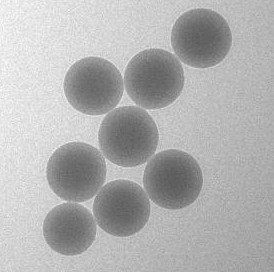
\includegraphics[height=2.25cm]{psbeads} \\
				{\footnotesize Particles}
				\par
			}
		\end{column}

	\end{columns}
	
	\vspace{1cm}
	
	\begin{columns}[t]
		\begin{column}[T]{\paperwidth/5}
			{\centering
				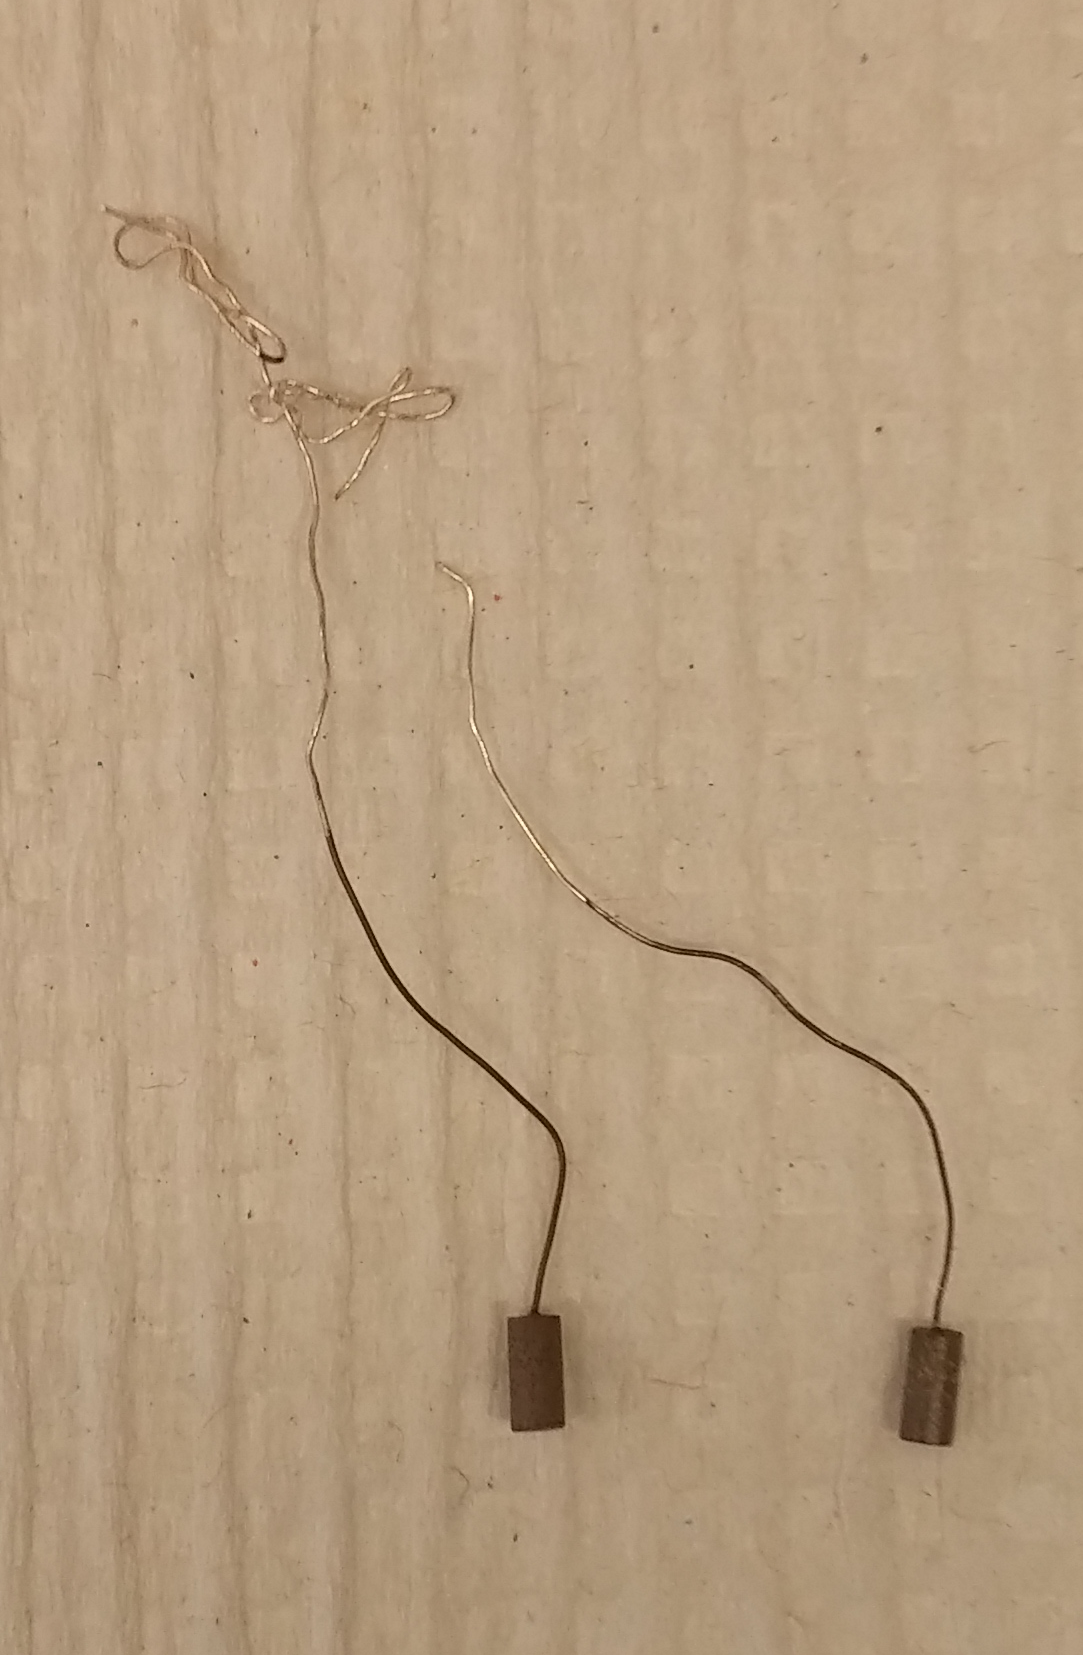
\includegraphics[height=2.25cm]{photo/electrodes.png} \\
				{\footnotesize Ag-AgCl electrodes}
				\par
			}
		\end{column}
		
		
		\begin{column}[T]{.6\paperwidth}
			{\centering
				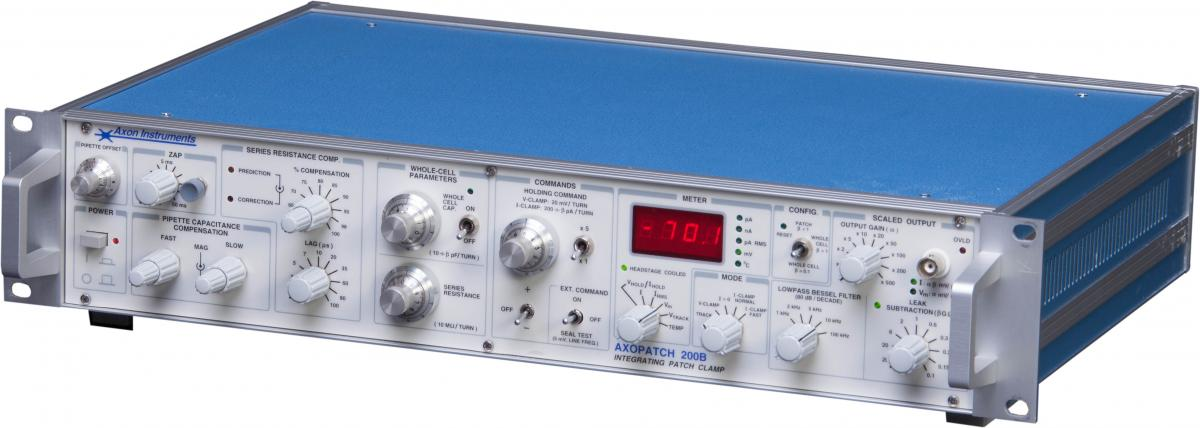
\includegraphics[height=2.25cm]{photo/axon200b} \\
				Voltage amplifier + current recorder
				\par
			}
		\end{column}
	

	\end{columns}




% 	
% 
% 
% 	\begin{center}
% 		\begin{figure}
% 		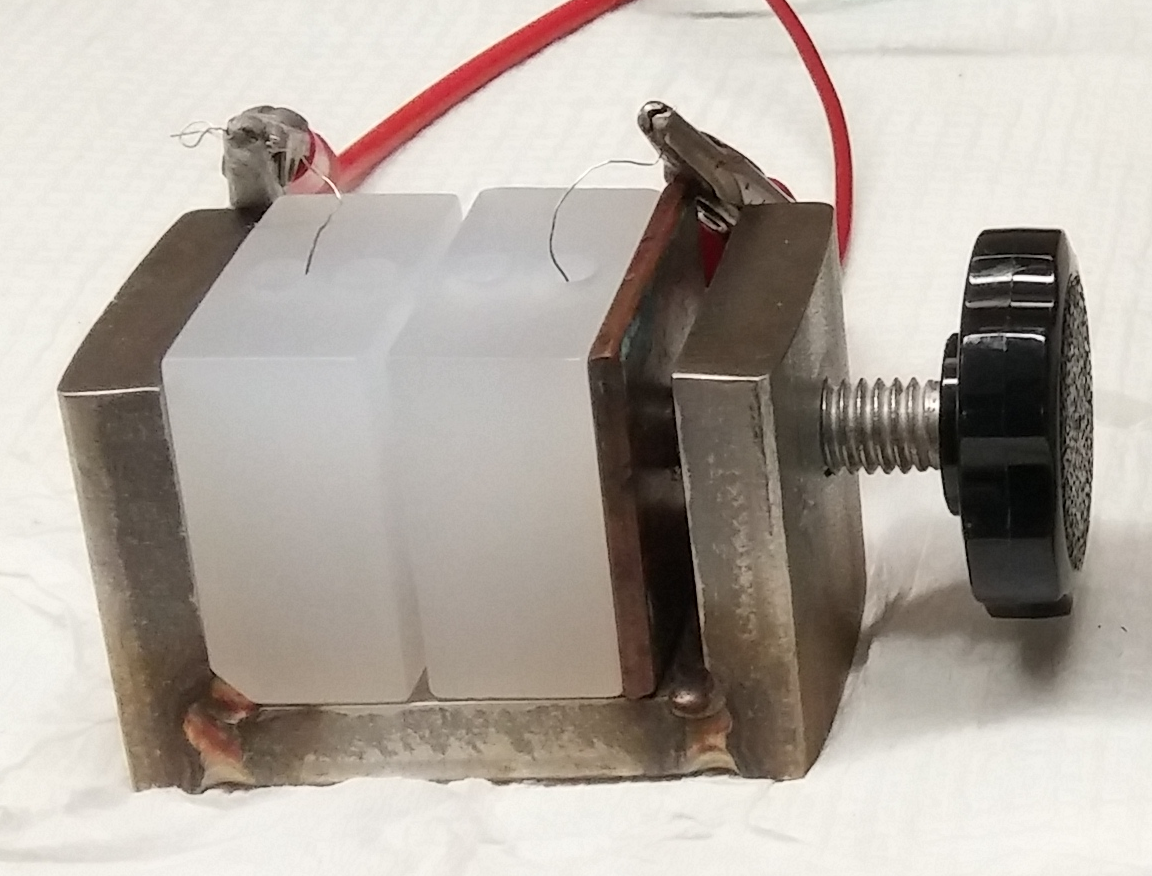
\includegraphics[height=2.25cm]{photo/conductivitycell.png}
% 		\caption{asdf}
% 		\end{figure}
% 		\hspace{.35cm}
%  		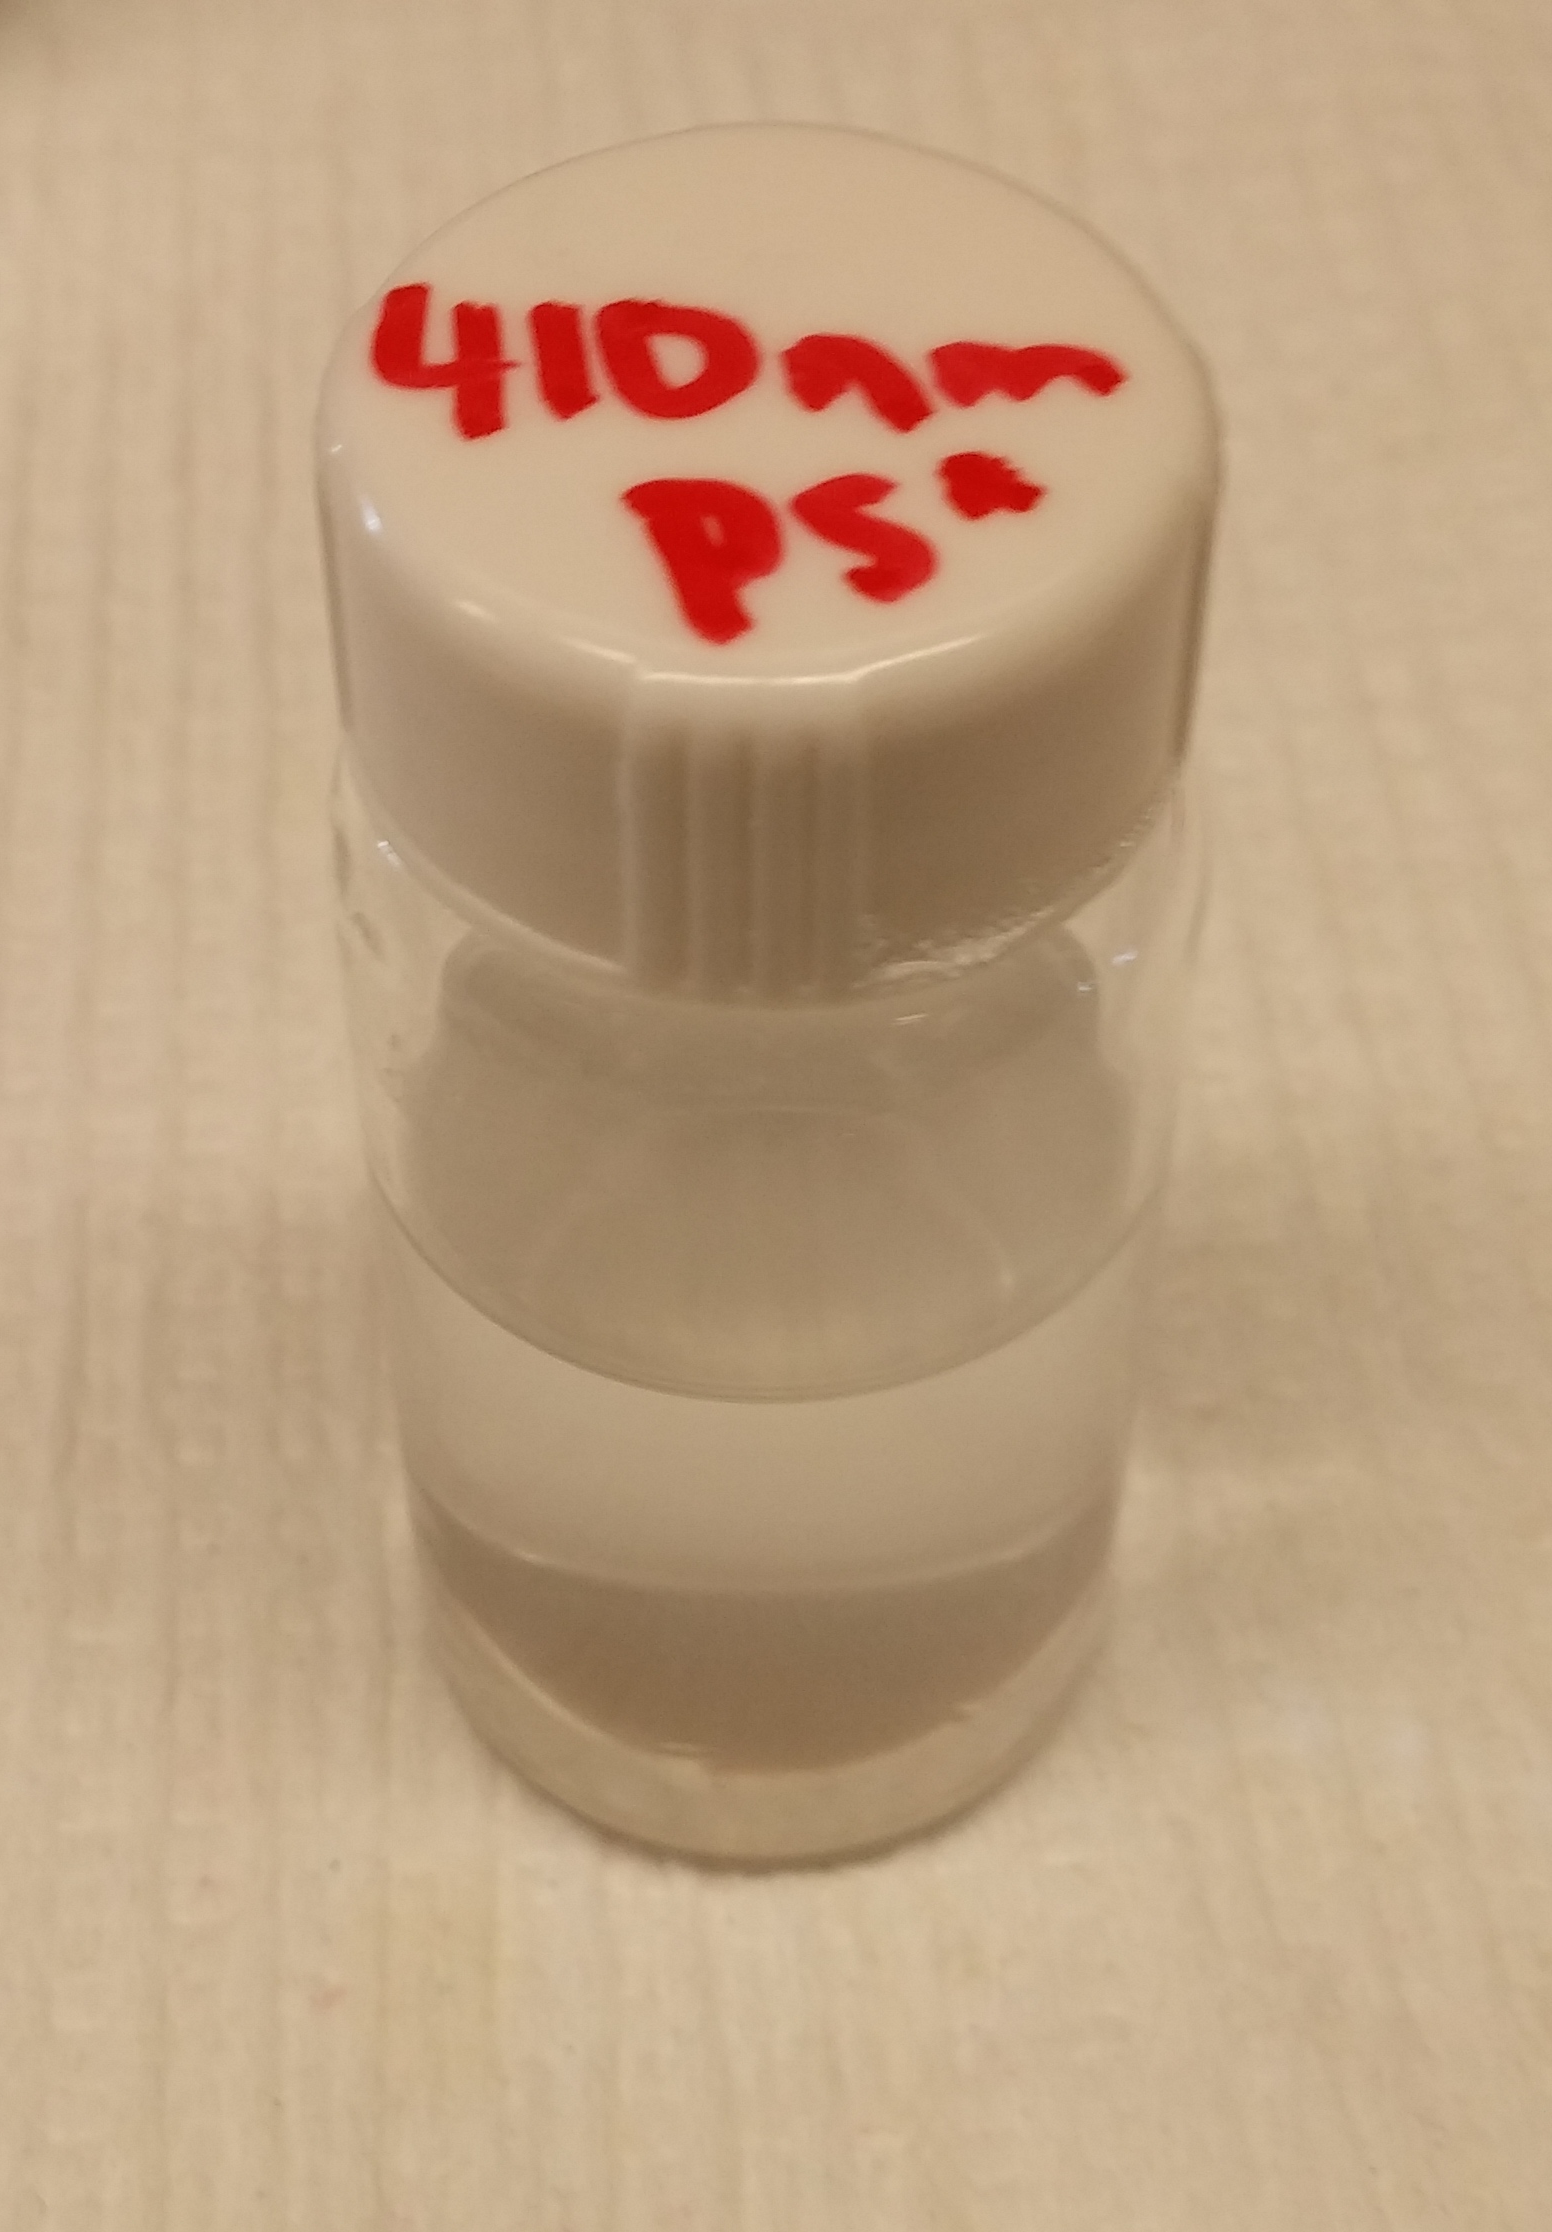
\includegraphics[height=2.25cm]{photo/solution.png}
%  		\hspace{.35cm}
%  		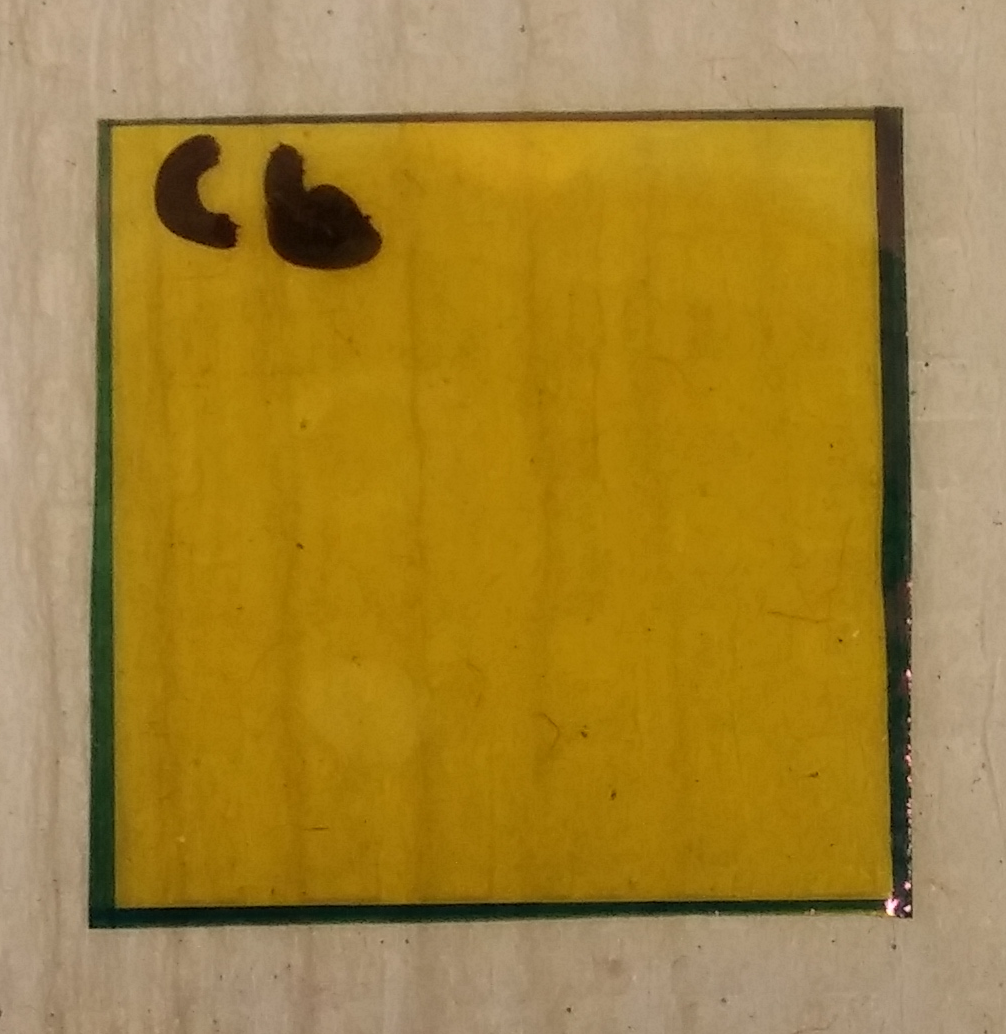
\includegraphics[height=2.25cm]{photo/membrane.png}
%  		\hspace{.35cm}
%  		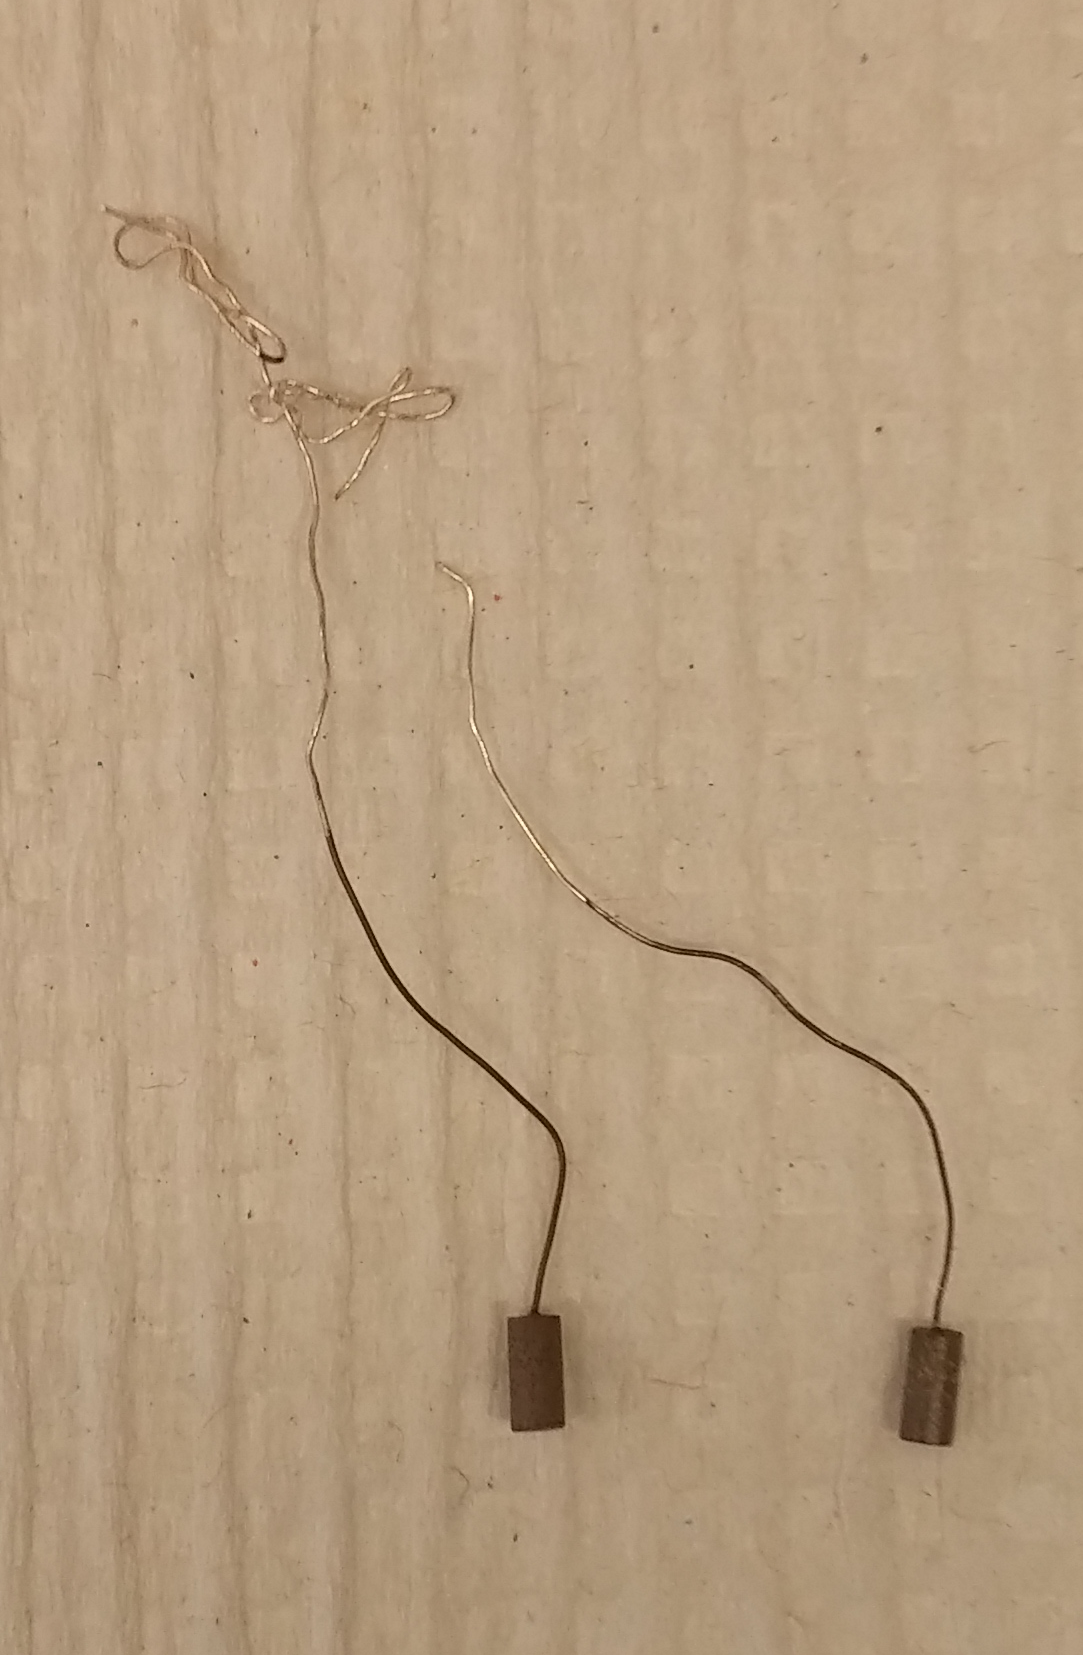
\includegraphics[height=2.25cm]{photo/electrodes.png}
%  		\hspace{.35cm}
% 	\end{center}

\end{frame}

%%%%%%%%%%%%%%%%%%%%%%%%%%%%%%%%%%%%%%%%%%%%%%%%%%%%%%%%%%%%%%%%%%%%%%%%%%%%%%%%%%%%%%%%%%%%%%%%%%%%%%%%%%%%%%%%%%%%%%%%%%%%
% Resistive pulse background---electrostatic boundary conditions
%%%%%%%%%%%%%%%%%%%%%%%%%%%%%%%%%%%%%%%%%%%%%%%%%%%%%%%%%%%%%%%%%%%%%%%%%%%%%%%%%%%%%%%%%%%%%%%%%%%%%%%%%%%%%%%%%%%%%%%%%%%%

\begin{frame}[c]{Resistive pulse sensing}
	{\centering
		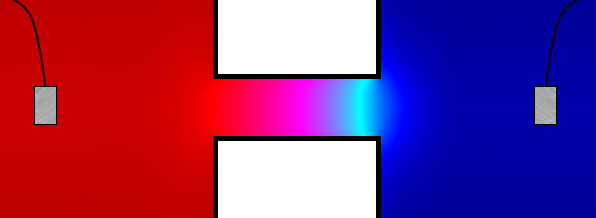
\includegraphics[width=0.9\paperwidth]{comsol/voltage.png}
		\par
	}
\end{frame}

%%%%%%%%%%%%%%%%%%%%%%%%%%%%%%%%%%%%%%%%%%%%%%%%%%%%%%%%%%%%%%%%%%%%%%%%%%%%%%%%%%%%%%%%%%%%%%%%%%%%%%%%%%%%%%%%%%%%%%%%%%%%
% Resistive pulse background---electrostatic boundary conditions
%%%%%%%%%%%%%%%%%%%%%%%%%%%%%%%%%%%%%%%%%%%%%%%%%%%%%%%%%%%%%%%%%%%%%%%%%%%%%%%%%%%%%%%%%%%%%%%%%%%%%%%%%%%%%%%%%%%%%%%%%%%%

\begin{frame}[c]{Resistive pulse sensing---electrostatic boundary conditions}
	{\centering
		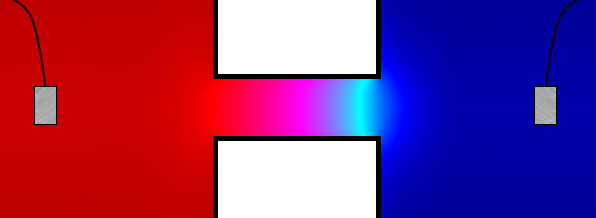
\includegraphics[width=0.9\paperwidth]{comsol/voltage.png}
		\par
	}
\end{frame}


%%%%%%%%%%%%%%%%%%%%%%%%%%%%%%%%%%%%%%%%%%%%%%%%%%%%%%%%%%%%%%%%%%%%%%%%%%%%%%%%%%%%%%%%%%%%%%%%%%%%%%%%%%%%%%%%%%%%%%%%%%%%
% Resistive pulse background---ion transport
%%%%%%%%%%%%%%%%%%%%%%%%%%%%%%%%%%%%%%%%%%%%%%%%%%%%%%%%%%%%%%%%%%%%%%%%%%%%%%%%%%%%%%%%%%%%%%%%%%%%%%%%%%%%%%%%%%%%%%%%%%%%

\tikzset{cross/.style={cross out, draw=black, minimum size=2*(#1-\pgflinewidth), inner sep=0pt, outer sep=0pt},
%default radius will be 1pt. 
cross/.default={1pt}}



\begin{frame}[c]{Resistive pulse sensing---ion transport}
	\begin{itemize}
		\item Ion transport is driven by \textbf{diffusion}, \textbf{convection}, and \textbf{electric migration}
		\item \underline{Diffusion}: Average flow of ions from high to low concentration
		\item \underline{Convection}: Ions move with the fluid/solvent
		\item \underline{Electrical migration}: Ions move in electric field
	\end{itemize}
	\only<1>{
		$$ \vec{J}_{i}=\underbrace{z_{i}eD_{i}\nabla c_{i}}_{\mathrm{diffusion}}+\overbrace{z_{i}ec_{i}\vec{u}}^{\mathrm{convection}}+\underbrace{z_{i}ec_{i}\mu_{i}\vec{E}}_{\mathrm{migration}} $$
	}
	\only<2>{
		$$ \vec{J}_{i}=\underbrace{\xcancel{z_{i}eD_{i}\nabla c_{i}}}_{\mathrm{diffusion}}+\overbrace{\xcancel{z_{i}ec_{i}\vec{u}}}^{\mathrm{convection}}+\underbrace{z_{i}ec_{i}\mu_{i}\vec{E}}_{\mathrm{migration}} $$
	}
	
	$$ I=\sum_{i}\iint_{S}\vec{J_{i}}\cdot \hat{n}dS $$
	
	% xs over two terms in equation
	\onslide<2>{
		\begin{tikzpicture}[]
			\draw(300,25) node[cross=10pt,red] {};
			\draw(1,0) node[cross=10pt,red] {};
		\end{tikzpicture}
	}

\end{frame}




%%%%%%%%%%%%%%%%%%%%%%%%%%%%%%%%%%%%%%%%%%%%%%%%%%%%%%%%%%%%%%%%%%%%%%%%%%%%%%%%%%%%%%%%%%%%%%%%%%%%%%%%%%%%%%%%%%%%%%%%%%%%
% Rods title slide
%%%%%%%%%%%%%%%%%%%%%%%%%%%%%%%%%%%%%%%%%%%%%%%%%%%%%%%%%%%%%%%%%%%%%%%%%%%%%%%%%%%%%%%%%%%%%%%%%%%%%%%%%%%%%%%%%%%%%%%%%%%%


\begin{frame}[c]{}
	\begin{center}
		\textbf{Resistive pulse sensing of high-aspect ratio particles}
	\end{center}
\end{frame}




%%%%%%%%%%%%%%%%%%%%%%%%%%%%%%%%%%%%%%%%%%%%%%%%%%%%%%%%%%%%%%%%%%%%%%%%%%%%%%%%%%%%%%%%%%%%%%%%%%%%%%%%%%%%%%%%%%%%%%%%%%%%
% Rods motivation slide
%%%%%%%%%%%%%%%%%%%%%%%%%%%%%%%%%%%%%%%%%%%%%%%%%%%%%%%%%%%%%%%%%%%%%%%%%%%%%%%%%%%%%%%%%%%%%%%%%%%%%%%%%%%%%%%%%%%%%%%%%%%%


\begin{frame}[c]{High-aspect ratio resistive pulse sensing---motivation}
 	\begin{itemize}
 		\item Aspherical particles are ubiquitous in biology---e.g., many viruses and bacteria are approximately rod-shaped
 	\end{itemize}


	\begin{columns}[t]
		\begin{column}[T]{2.5in}
			{\centering
				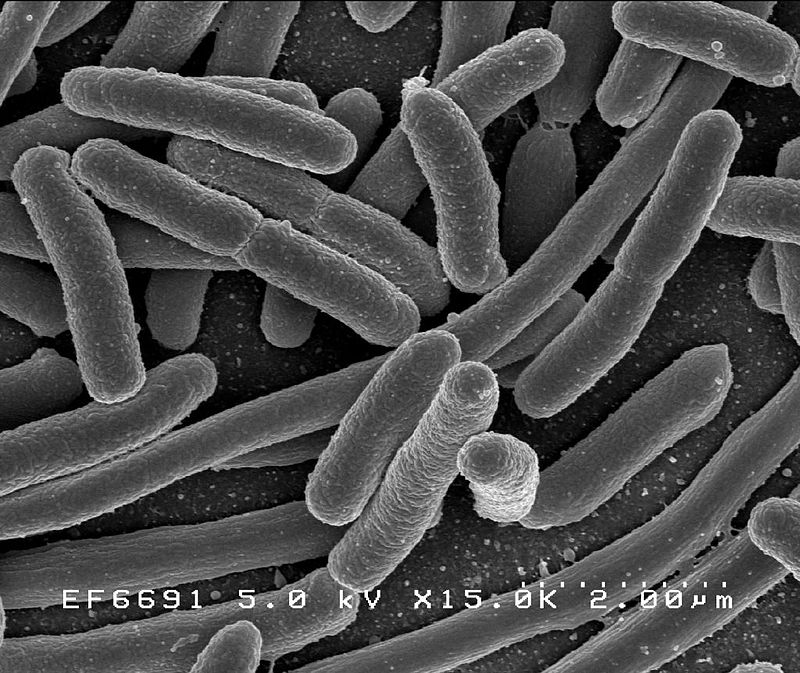
\includegraphics[height=2.25cm]{ecoli} \\
				e. coli \\
				$L\sim \SI{2}{\mu m}$ \\
				\par
			}
		\end{column}
		
		
		\begin{column}[T]{2.5in}
			{\centering
				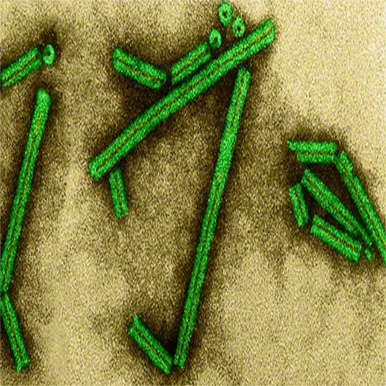
\includegraphics[height=2.25cm]{tobaccomosaicvirus} \\
				tobacco mosaic virus \\
				$L\sim \SI{300}{nm}$ \\
				\par
			}
		\end{column}
	

	\end{columns}

	\begin{itemize}
		\item The ability to measure particle shape is highly desirable for sensing applications
 		\item How can we extend RP sensing to measure length in addition to volume?
 	\end{itemize}
	

\end{frame}




%%%%%%%%%%%%%%%%%%%%%%%%%%%%%%%%%%%%%%%%%%%%%%%%%%%%%%%%%%%%%%%%%%%%%%%%%%%%%%%%%%%%%%%%%%%%%%%%%%%%%%%%%%%%%%%%%%%%%%%%%%%%
% Resistive pulse in non-constant width pores
%%%%%%%%%%%%%%%%%%%%%%%%%%%%%%%%%%%%%%%%%%%%%%%%%%%%%%%%%%%%%%%%%%%%%%%%%%%%%%%%%%%%%%%%%%%%%%%%%%%%%%%%%%%%%%%%%%%%%%%%%%%%

\begin{frame}[c]{Resistive pulse in non-constant width pores}
	\begin{itemize}
		\item Consider the RP amplitude for translocation through non-uniform pores
	\end{itemize}
	$$ \Delta R\left(z'\right)=\frac{\rho}{\pi}\left[\int_{z=z'}^{z=z'+l_{p}}\left(\frac{1}{r_{P}^{2}\left(z\right)-s_{p}^{2}\left(z\right)}-\frac{1}{r_{P}\left(z\right)^{2}}\right)dz\right] $$
	\begin{itemize}
		\item RP amplitude is a function of the pore geometry \textbf{local to the particle's position}
		\item Particles map the interior of the pore during translocation with their RP signal!
	\end{itemize}
	
	{\centering
		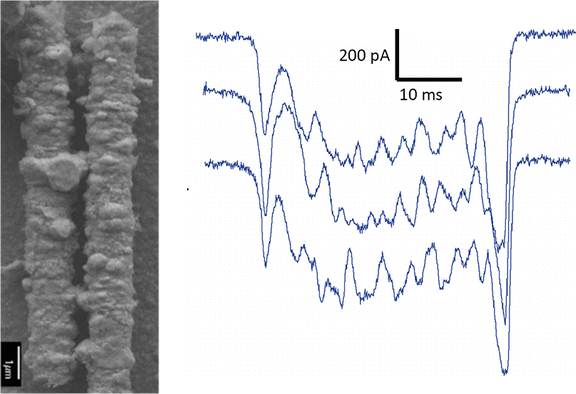
\includegraphics[width=2in]{particlesreveal.png} \\
		\par
	}

	
\end{frame}


%%%%%%%%%%%%%%%%%%%%%%%%%%%%%%%%%%%%%%%%%%%%%%%%%%%%%%%%%%%%%%%%%%%%%%%%%%%%%%%%%%%%%%%%%%%%%%%%%%%%%%%%%%%%%%%%%%%%%%%%%%%%
% RP signal resolution
%%%%%%%%%%%%%%%%%%%%%%%%%%%%%%%%%%%%%%%%%%%%%%%%%%%%%%%%%%%%%%%%%%%%%%%%%%%%%%%%%%%%%%%%%%%%%%%%%%%%%%%%%%%%%%%%%%%%%%%%%%%%

\begin{frame}[c]{RP signal resolution}
	
	\vspace{-.1in}
	\begin{itemize}
		\item Particles map pore interiors with a length-dependent resolution
		\item If a particle has length smaller than the characteristic length scale of channel irregularities, the produced signal is a high-resolution mapping
		\item Particles with lengths longer than characteristic length scale of channel irregularities produce low-resolution mappings
	\end{itemize}
	
	
	
	\begin{columns}[t]
		
	
		\begin{column}[T]{2.25in}
			{\centering
				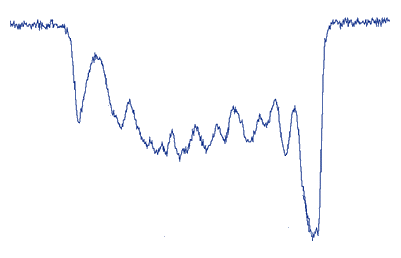
\includegraphics[height=1in]{plain_signal.png} \\
				Short particle \\
			}
		\end{column}
		  
		\begin{column}[T]{2.25in}
			{\centering
				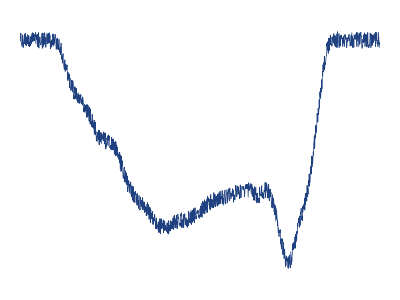
\includegraphics[height=1.in,width=2in]{mystery_plain_signal_3.png} \\
				Long particle (simulated) \\
			}
		\end{column}

	\end{columns}
	\vspace{.2in}
	\textcolor{negativered}{\textbf{Can we use this knowledge to measure particle length???}}

	%$$ \Delta R\left(z'\right)=\frac{\rho}{\pi}\left[\int_{z=z'}^{z=z'+l_{p}}\left(\frac{1}{r_{P}^{2}\left(z\right)-s_{p}^{2}\left(z\right)}-\frac{1}{r_{P}^{2}\left(z\right)}\right)dz\right] $$

	
	
	
	

\end{frame}


%%%%%%%%%%%%%%%%%%%%%%%%%%%%%%%%%%%%%%%%%%%%%%%%%%%%%%%%%%%%%%%%%%%%%%%%%%%%%%%%%%%%%%%%%%%%%%%%%%%%%%%%%%%%%%%%%%%%%%%%%%%%
% Qualitative length comparison
%%%%%%%%%%%%%%%%%%%%%%%%%%%%%%%%%%%%%%%%%%%%%%%%%%%%%%%%%%%%%%%%%%%%%%%%%%%%%%%%%%%%%%%%%%%%%%%%%%%%%%%%%%%%%%%%%%%%%%%%%%%%

\begin{frame}[c]{Qualitative length comparison}
	\vspace{.3in}
	\begin{picture}(0,0)(0,0)
		\put(0,-25)
		{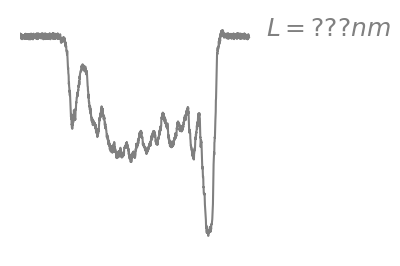
\includegraphics[width=3.75cm]{mystery_plain_signal_2.png}}
		\put(0,-125)
		{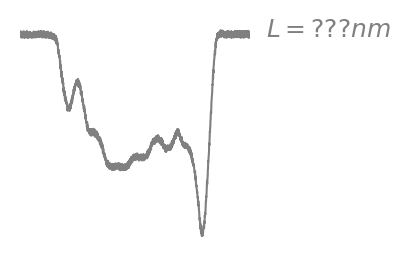
\includegraphics[width=3.75cm]{mystery_plain_signal.png}}
		\put(200,-125)
		{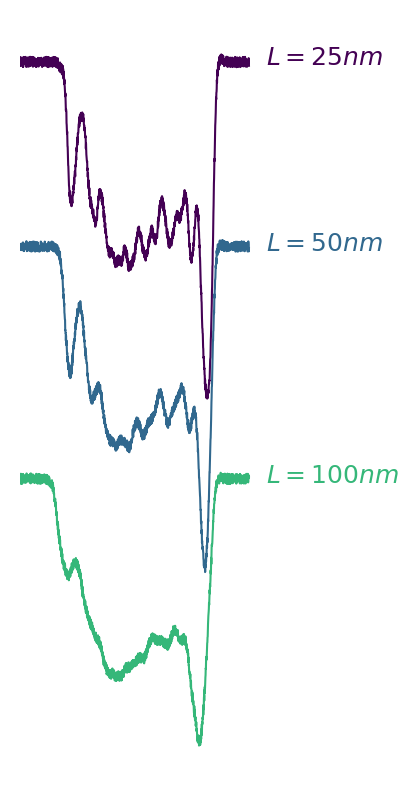
\includegraphics[height=7cm]{plain_signals_smoothed.png}}
	\end{picture}
	
	\begin{tikzpicture}[overlay, x=1cm,y=1cm]
		% Coordinates
		\coordinate (x1) at (2.5, -2.5) ;
		\coordinate (x2) at (5.5, -2.5) ;
		\coordinate (x3) at (5.5, -.5) ;
		\coordinate (x4) at (7.25, -.5) ;
		
		
		\coordinate (x5) at (2.5, 1.) ;
		\coordinate (x6) at (5.5, 1.) ;
		\coordinate (x7) at (5.5, 2.95) ;
		\coordinate (x8) at (7.25, 2.95) ;

		% Text hack
		\node[right] (mag) at (0.25,3.5) {\footnotesize\textcolor{porestatsblack}{Unidentified particles}};
		\node[right] (mag) at (7.25,3.5) {\footnotesize\textcolor{porestatsblack}{Tracer particles}};


		    		    
		% Arrow
		\path[draw=gray1,thick,->] (x1) to[straight] (x2) to[straight] (x3) to[straight] (x4);
		\path[draw=gray1,thick,->] (x5) to[straight] (x6) to[straight] (x7) to[straight] (x8);


			
	\end{tikzpicture}
	

\end{frame}


%%%%%%%%%%%%%%%%%%%%%%%%%%%%%%%%%%%%%%%%%%%%%%%%%%%%%%%%%%%%%%%%%%%%%%%%%%%%%%%%%%%%%%%%%%%%%%%%%%%%%%%%%%%%%%%%%%%%%%%%%%%%
% Quantitative length measurement
%%%%%%%%%%%%%%%%%%%%%%%%%%%%%%%%%%%%%%%%%%%%%%%%%%%%%%%%%%%%%%%%%%%%%%%%%%%%%%%%%%%%%%%%%%%%%%%%%%%%%%%%%%%%%%%%%%%%%%%%%%%%

\begin{frame}[c]{Reexpressing the RP amplitude of a long particle in terms of shorter particles}
	
	
	{\footnotesize
	Because resistances add in series, we can express the RP amplitude of a long particle as a sum over the RP amplitudes of shorter particles
	}
	
	
	{\scriptsize
		\begin{equation*}
			\begin{split}
				\Delta R_{l}\left(z\right) &= \frac{\rho}{\pi}\left[\int_{z}^{z+l_{p}}\left(\frac{1}{r_{P}^{2}\left(z'\right)-s_{p}^{2}\left(z'\right)}-\frac{1}{r_{P}^{2}\left(z'\right)}\right)dz'\right] \\
				&= \frac{\rho}{\pi}\left[\int_{z}^{z+l_{s}}\left(\frac{1}{r_{P}^{2}\left(z'\right)-s_{p}^{2}\left(z'\right)}-\frac{1}{r_{P}^{2}\left(z'\right)}\right)dz'\right. \\
				&+ \int_{z+l_{s}}^{z+2l_{s}}\left(\frac{1}{r_{P}^{2}\left(z'\right)-s_{p}^{2}\left(z'\right)}-\frac{1}{r_{P}^{2}\left(z'\right)}\right)dz + ...\\
				&+ \left.\int_{z+\left(n-1\right)l_{s}}^{z+nl_{s}}\left(\frac{1}{r_{P}^{2}\left(z'\right)-s_{p}^{2}\left(z'\right)}-\frac{1}{r_{P}^{2}\left(z'\right)}\right)dz'\right] \\
				&= \sum_{i=0}^{n-1}\frac{\rho}{\pi}\left[\int_{z+il_{s}}^{z+\left(i+1\right)l_{s}}\left(\frac{1}{r^{2}_{P}\left(z'\right)-s^{2}_{p}\left(z'\right)}-\frac{1}{r_{P}^{2}\left(z'\right)}\right)dz'\right] \\
				&= \sum_{i=0}^{n-1}\Delta R_{s}\left(z+il_{s}\right)
			\end{split}
		\end{equation*}
	}


		



\end{frame}




%%%%%%%%%%%%%%%%%%%%%%%%%%%%%%%%%%%%%%%%%%%%%%%%%%%%%%%%%%%%%%%%%%%%%%%%%%%%%%%%%%%%%%%%%%%%%%%%%%%%%%%%%%%%%%%%%%%%%%%%%%%%
% Quantitative length measurement
%%%%%%%%%%%%%%%%%%%%%%%%%%%%%%%%%%%%%%%%%%%%%%%%%%%%%%%%%%%%%%%%%%%%%%%%%%%%%%%%%%%%%%%%%%%%%%%%%%%%%%%%%%%%%%%%%%%%%%%%%%%%

\begin{frame}[c]{Quantitative length measurement}
	
	\begin{columns}[t]
		\begin{column}[T]{2.25in}
			{\footnotesize
				Reexpressing the amplitude of long particles in terms of amplitude of short particles suggests a means of measuring length \\
				\vspace{.2in}
				We perform a convolution of the RP amplitude signals of shorter particles over various length intervals \\
				\vspace{.2in}
				Then, we select the length for which the convolved signal had the greatest similarity to the raw signal of the unknown particle
			}
		\end{column}
		
		\begin{column}[T]{2.25in}
			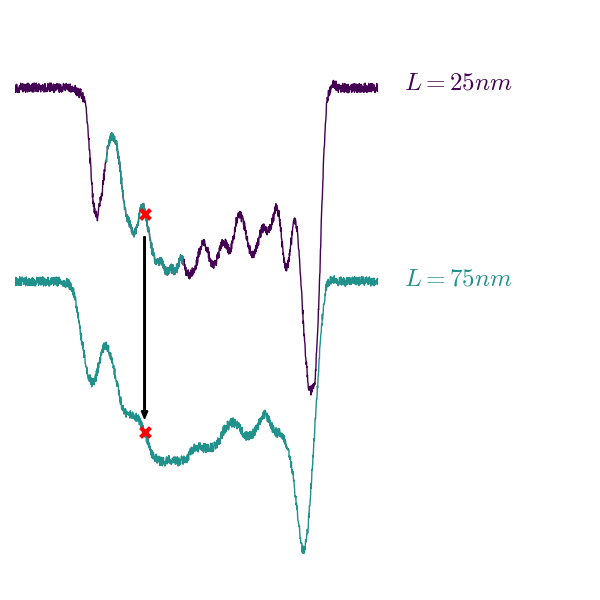
\includegraphics[width=2.25in]{moving_average_process.png}
		\end{column}


	\end{columns}
\end{frame}





%%%%%%%%%%%%%%%%%%%%%%%%%%%%%%%%%%%%%%%%%%%%%%%%%%%%%%%%%%%%%%%%%%%%%%%%%%%%%%%%%%%%%%%%%%%%%%%%%%%%%%%%%%%%%%%%%%%%%%%%%%%%
% Length measurement experimental platform
%%%%%%%%%%%%%%%%%%%%%%%%%%%%%%%%%%%%%%%%%%%%%%%%%%%%%%%%%%%%%%%%%%%%%%%%%%%%%%%%%%%%%%%%%%%%%%%%%%%%%%%%%%%%%%%%%%%%%%%%%%%%

\begin{frame}[c]{Length measurement experimental test}
	\begin{itemize}
		\item Resistive pulse experiments were conducted with PET membranes
		\item Three types of particles were tested
		\begin{itemize}
			\item $\SI{400}{nm}$ polystyrene beads  (`spheres')
			\item $\SI{590}{nm}$ rods (`short rods')
			\item $\SI{1920}{nm}$ rods (`long rods')
		\end{itemize}
	\end{itemize}
	
	\begin{columns}[t]
		\begin{column}[T]{2.25in}
			{\centering
				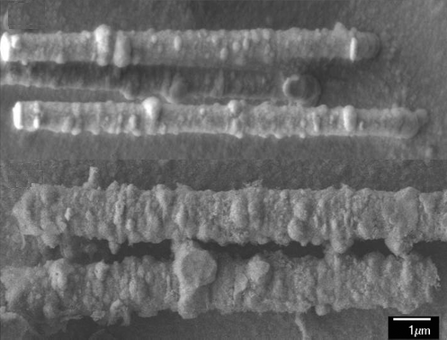
\includegraphics[height=0.75in]{PET.png} \\
				PET pore metal replica \\
				\par
			}
		\end{column}
		
		\begin{column}[T]{2.25in}
			{\centering
				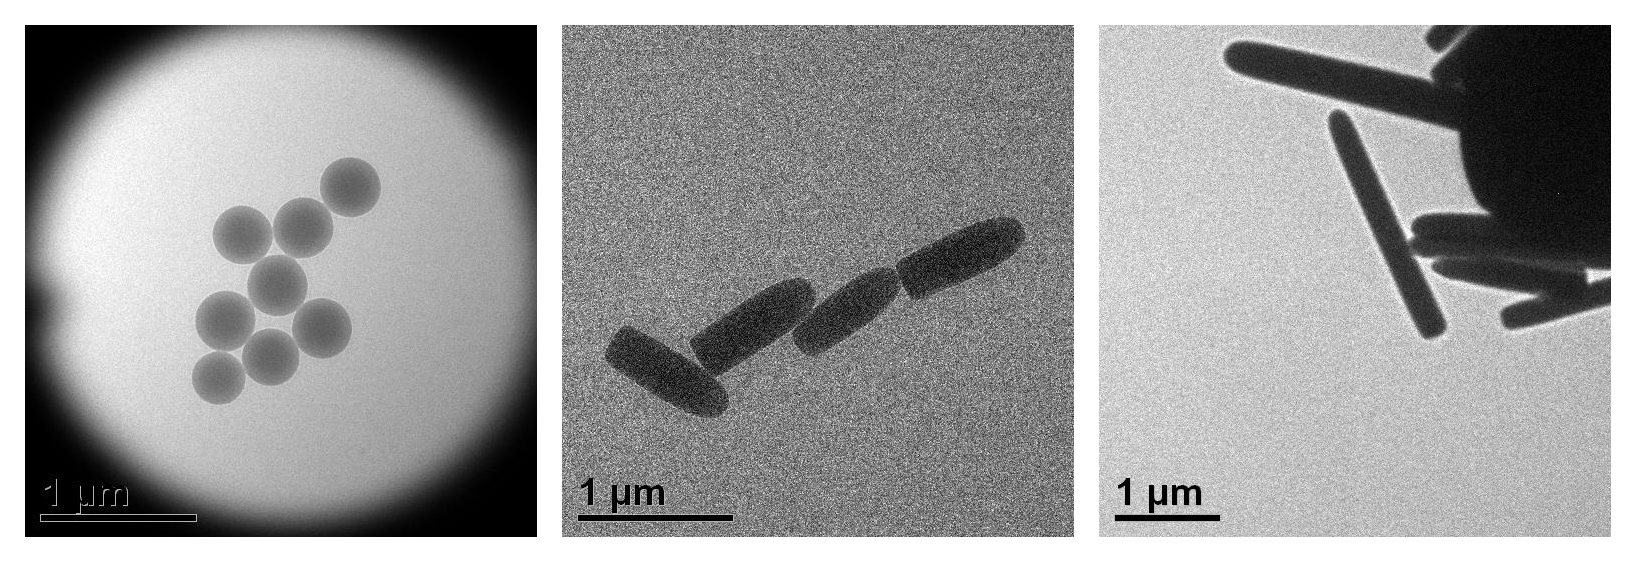
\includegraphics[height=0.75in]{particles.png} \\
				Nanoparticles \\
				\par				
			}
		\end{column}

	\end{columns}



\end{frame}



%%%%%%%%%%%%%%%%%%%%%%%%%%%%%%%%%%%%%%%%%%%%%%%%%%%%%%%%%%%%%%%%%%%%%%%%%%%%%%%%%%%%%%%%%%%%%%%%%%%%%%%%%%%%%%%%%%%%%%%%%%%%
% Length measurement experimental platform
%%%%%%%%%%%%%%%%%%%%%%%%%%%%%%%%%%%%%%%%%%%%%%%%%%%%%%%%%%%%%%%%%%%%%%%%%%%%%%%%%%%%%%%%%%%%%%%%%%%%%%%%%%%%%%%%%%%%%%%%%%%%

\begin{frame}[c]{Particles to scale}
	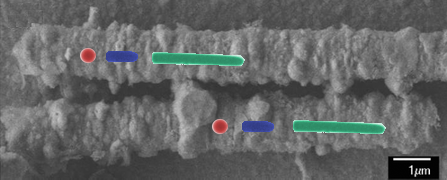
\includegraphics[width=4.5in]{particles_real_size.png}
\end{frame}




%%%%%%%%%%%%%%%%%%%%%%%%%%%%%%%%%%%%%%%%%%%%%%%%%%%%%%%%%%%%%%%%%%%%%%%%%%%%%%%%%%%%%%%%%%%%%%%%%%%%%%%%%%%%%%%%%%%%%%%%%%%%
% Results---PET7
%%%%%%%%%%%%%%%%%%%%%%%%%%%%%%%%%%%%%%%%%%%%%%%%%%%%%%%%%%%%%%%%%%%%%%%%%%%%%%%%%%%%%%%%%%%%%%%%%%%%%%%%%%%%%%%%%%%%%%%%%%%%

\begin{frame}[c]{Results---PET7 raw events}
	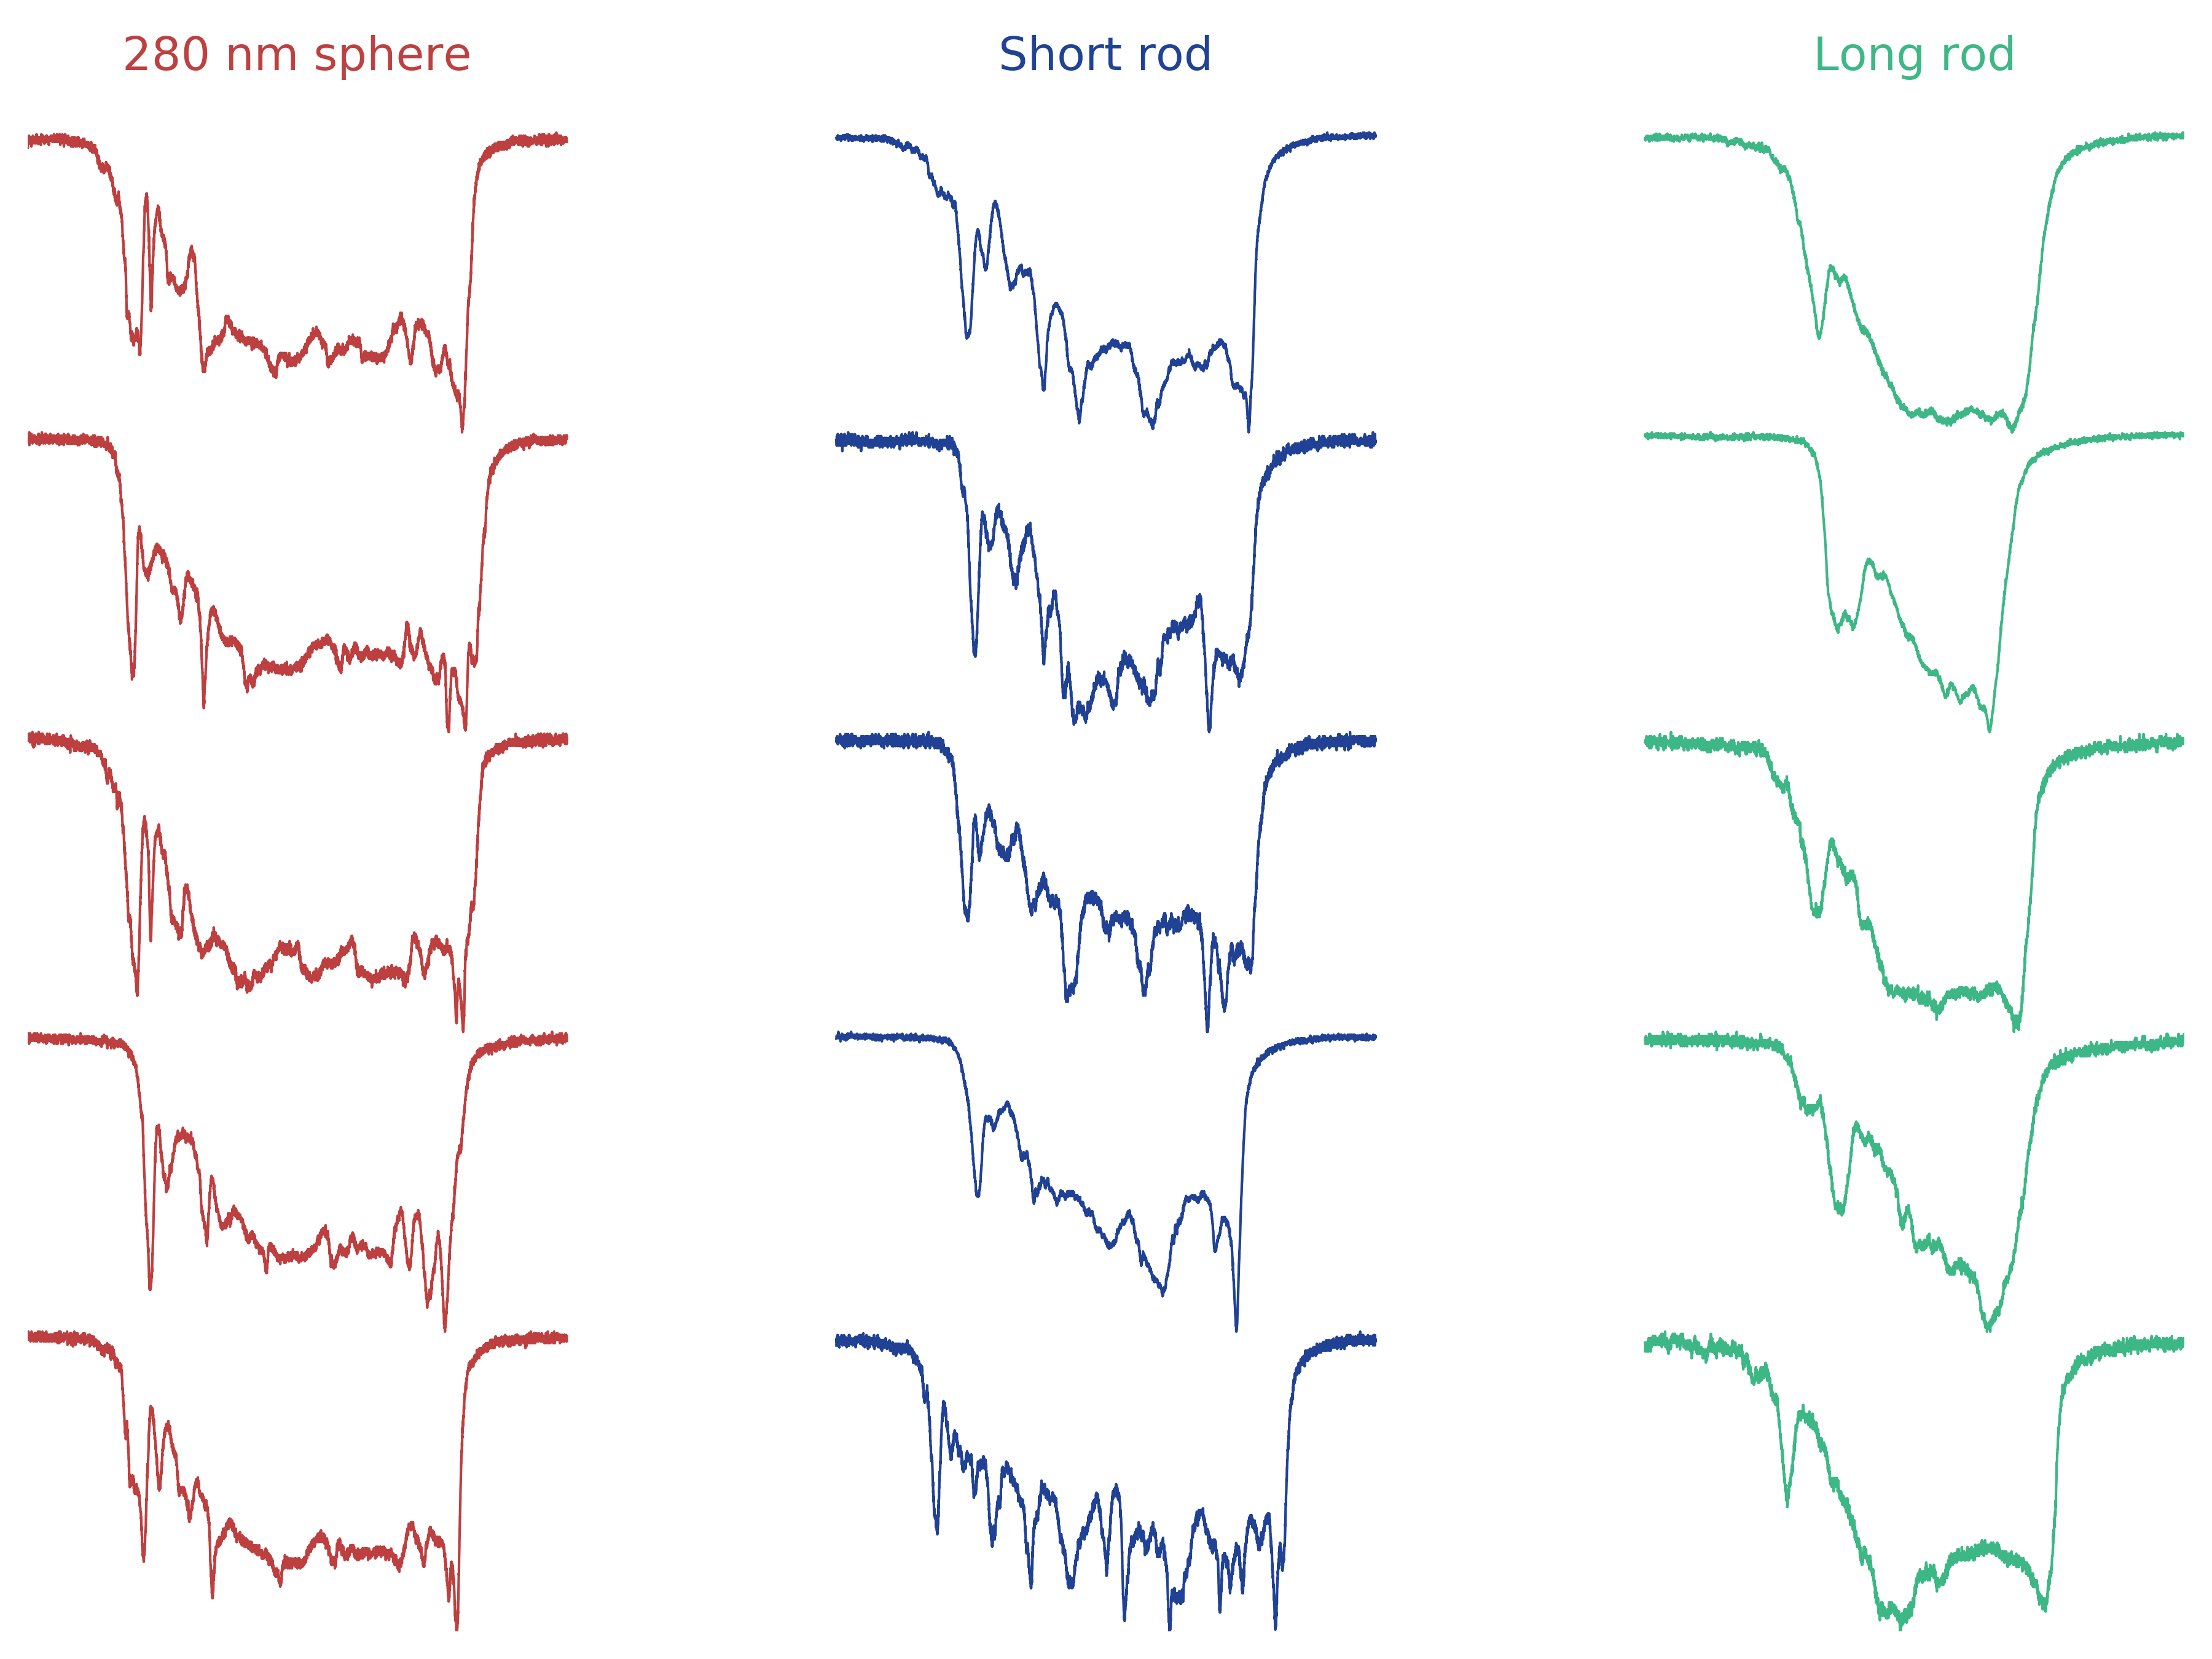
\includegraphics[width=4.5in]{PET7_raw.png}
\end{frame}